 %%
%% Beginning of file 'sample.tex'
%%
%% Modified 2005 December 5
%%
%% This is a sample manuscript marked up using the
%% AASTeX v5.x LaTeX 2e macros.

%% The first piece of markup in an AASTeX v5.x document
%% is the \documentclass command. LaTeX will ignore
%% any data that comes before this command.

%% The command below calls the preprint style
%% which will produce a one-column, single-spaced document.
%% Examples of commands for other substyles follow. Use
%% whichever is most appropriate for your purposes.
%%
%%\documentclass[12pt,preprint]{aastex}

%% manuscript produces a one-column, double-spaced document:

%\documentclass[manuscript]{aastex}

%% preprint2 produces a double-column, single-spaced document:

%\documentclass[preprint2]{aastex}

%% Sometimes a paper's abstract is too long to fit on the
%% title page in preprint2 mode. When that is the case,
%% use the longabstract style option.

 \documentclass[preprint2,longabstract]{aastex}
%% If you want to create your own macros, you can do so
%% using \newcommand. Your macros should appear before
%% the \begin{document} command.
%%
%% If you are submitting to a journal that translates manuscripts
%% into SGML, you need to follow certain guidelines when preparing
%% your macros. See the AASTeX v5.x Author Guide
%% for information.

\newcommand{\vdag}{(v)^\dagger}
\newcommand{\myemail}{skywalker@galaxy.far.far.away}

%% You can insert a short comment on the title page using the command below.

%\slugcomment{Not to appear in Nonlearned J., 45.}

%% If you wish, you may supply running head information, although
%% this information may be modified by the editorial offices.
%% The left head contains a list of authors,
%% usually a maximum of three (otherwise use et al.).  The right
%% head is a modified title of up to roughly 44 characters.
%% Running heads will not print in the manuscript style.

%\shorttitle{Collapsed Cores in Globular Clusters}
%\shortauthors{Djorgovski et al.}

%% This is the end of the preamble.  Indicate the beginning of the
%% paper itself with \begin{document}.

\begin{document}

%% LaTeX will automatically break titles if they run longer than
%% one line. However, you may use \\ to force a line break if
%% you desire.

\title{AKARI and Spinning Dust Emission\\
A look at microwave dust emission via the Infrared}

%% Use \author, \affil, and the \and command to format
%% author and affiliation information.
%% Note that \email has replaced the old \authoremail command
%% from AASTeX v4.0. You can use \email to mark an email address
%% anywhere in the paper, not just in the front matter.
%% As in the title, use \\ to force line breaks.

%\author{S. Djorgovski\altaffilmark{1,2,3} and Ivan R. King\altaffilmark{1}}
%\affil{Astronomy Department, University of California,
%    Berkeley, CA 94720}

\author{A. Bell, T. Onaka, F. Galliano, R. Wu, M. Hammonds, Y. Doi, D. Ishihara, M. Giard}
\affil{University of Tokyo,
   Bunkyo, Tokyo, Japan, 113-0033;}

\email{abell@astron.s.u-tokyo.ac.jp}



%% Notice that each of these authors has alternate affiliations, which
%% are identified by the \altaffilmark after each name.  Specify alternate
%% affiliation information with \altaffiltext, with one command per each
%% affiliation.

%\altaffiltext{1}{Visiting Astronomer, Cerro Tololo Inter-American Observatory.
%CTIO is operated by AURA, Inc.\ under contract to the National Science
%Foundation.}
%%\altaffiltext{3}{present address: Center for Astrophysics,
%    60 Garden Street, Cambridge, MA 02138}
%\altaffiltext{4}{Visiting Programmer, Space Telescope Science Institute}
%\altaffiltext{5}{Patron, Alonso's Bar and Grill}

%% Mark off your abstract in the ``abstract'' environment. In the manuscript
%% style, abstract will output a Received/Accepted line after the
%% title and affiliation information. No date will appear since the author
%% does not have this information. The dates will be filled in by the
%% editorial office after submission.

\begin{abstract}
%The anomalous microwave emission (AME) still lacks a coherent explanation. Both electric dipole emission by rapidly rotating dust (``spinning dust") and magnetic dipole emission by grains with magnetic inclusions (``magnetic dust") have emerged as theoretically plausible explanations. We explore the spinning dust angle. Specifically, the particular scenario in which spinning polycyclic aromatic hydrocarbon molecules (PAHs) are the dominant carriers of the AME. We use AKARI/Infrared Camera (IRC), due to its thorough PAH-band coverage, to analyze 98 regions showing evidence of AME. Also in the mid-infrared, we include the PAH-tracing bands of IRAS, WISE, and DIRBE (around 12 microns), for comparison to the pre-release IRC data. We supplement the MIR data with AKARI Far Infrared Surveyor (FIS), and Planck High Frequency Instrument (HFI) bands at 857 and 545~GHz, and IRAS to constrain the full dust thermal spectral energy distribution (SED). We carry out a dust SED fitting and find no preferential relationship between estimates of PAH abundance and the AME. At best, they PAH-dominated bands correlate with AME as well as the band s tracing the peak thermal dust emission. The results are consistent with previous studies in that the AME has a clear connection to interstellar dust, but a conclusive link to any particular population of dust is unapparent.
\end{abstract}


\keywords{AME, spinning dust, PAH bands, AKARI}


\maketitle
%\tableofcontents
\section{Introduction}

     Since its first detection in early microwave surveys , the anomalous microwave emission/foreground (AME) has been found to be a widespread feature of the microwave Milky Way \citep{dickinson13r}. \cite{kogut96,deoliveiracosta97,leitch98} showed that the AME correlates very well with infrared emission from dust, via COBE/DIRBE and IRAS far-IR maps. However there is still much mystery, except that the most likely source of the AME is interstellar dust \citep{ysard10a,tibbs11,hensley16}.

     From the observed spatial correlation between AME and dust emerged two prevailing hypotheses:

     1) Electric dipole emission by spinning small dust grains, a mechanism proposed in \cite{erickson57} and \cite{hoyle70}, with further discussion in \cite{ferrara94}. \cite{draine98b} give the earliest thorough description, with substantial updates contributed more recently by \cite{ysard10a}, \cite{ali-haimoud09}, \cite{hoang10} and several others. \cite{hensey17} propose that such small spinning grains may consist primarily of silicates, and that observational upper-bounds of nanosilicate abudance allows for such a scenario. \cite{dickinson13r} provide a detailed overview of AME and spinning dust literature.

     2) Magnetic dipole emission, caused by thermal fluctuations in grains with magnetic inclusions, proposed by \cite{draine99}.

     More recently, modeled spectra for potential candidate carriers have appeared in the literature: PAHs, grains with magnetic inclusions \citep{draine13, ali-haimoud14, hoang16a}.

    A third, but not widely accepted, possible explanation for AME is discussed in \cite{jones09}. They have suggested that the emissivity of dust, in the spectral range related to AME, could contain features caused by low temperature solid-state structural transitions.


     Although spinning dust need not be the only emission mechanism, the photometric signature of the AME, has so far been commonly explained via spinning dust parameters \citep{ysard11,ali-haimoud10}. In this paper, we explore the case that the AME signature arises from spinning dust emission. If the AME is carried by spinning dust, the carrier should be small enough that it can be rotationally excuted to frequencies in the range of 10-40~GHz, and must have a permanent electric dipole. Within contemporary dust SED models, only the polycyclic aromatic hydrocarbon family of molecules (PAHs), or nanoscale amorphous carbon dust fit these criteria. Those PAHs which have a permanent electric dipole (i.e. coranulene, but not symmetric molecules like coronene), can emit rotationally. However the carrier need not be carbon-based. Indeed, \cite{hensley17a} claim that AME can be explained without carbonaceous carriers, using only spinning nanosilicates.

     While neither nanosilicates nor PAHs have been conclusively identified in the ISM, mid-infrared features associated with PAH-like aromatic materials have been observed. In fact, ``the PAH features'' are ubiquitous in the ISM \citep{giard94,onaka96,onaka00}, such that the carriers must be abundant.  However \cite{andrews15} strongly argue for the  existence of a dominant ``grandPAH'' class, containing 20 to 30 PAH species. On the other hand, there has yet to be any detection of features related to nanosilicates. There is only an upper-bound from IRTS observations of \cite{onaka96} and calculations by \cite{li01}.

     Assuming a rotational emission model, the AME signature (consistent with continuum emission having a peak around 20 to 40~GHz ) implies very small oscillators (\textasciitilde{}10~nm). In any case, the PAH class of molecules are the only spinning dust candidate so far which show both: 1) Evidence of abundance in the ISM at IR wavelengths, and 2) A predicted range of dipole moments (on order of 1~debye), to produce the observed AME signature \citep{draine98b, lovas05, thorwirth07}. However, it should be noted that the current upper-bound on the abundance of nanosilicates, allows for a "spinning nanosilicate" explanation for the AME, as shown by \cite{hensley17a}. Due to the (apparently) continuous shape of the AME SED, a distribution of dipole moments and rotational velocities is needed, in a spinning dust scenario. Of course, the AME cannot simply be modeled by a distribution of carriers. Environmental factors must be considered.

     In the spinning dust model, there are several possible excitation factors for spinning dust. While the question of whether or not such small grains would be spinning at all is a bit trivial- a case in which grains had no angular momentum would be bizarre- for the grains to have rotational velocities high enough to create the observed AME, they must be subject to strong excitation mechansisms. The dominant factors that would be giving grains their spin, are broken down by \cite{draine11} into basically two categories: 1) Collisional excitation. 2) Radiative excitation, the sum of which could lead to sufficient rotational velocities for sufficiently small grains. However the extent of excitation will depend on environmental conditions, i.e. there will be more frequent encounters with ions and atoms in denser regions (so long as the density is not high enough to coagulate the small grains), and more excitation due to photon emission with increasing ISRF strength \citep{ali-haimoud09, ali-haimoud13}. One of the strongest potential excitation mechansims listed in \cite{draine11} is that of negatively charged grains interacting with ions. Thus not only must we consider environmental factors, grain composition and size, but also the ionization state of the carriers. (For example, ionizaed vs. neutral PAHs.) The dependence of the observed AME on ISM density is modeled by \cite{ali-haimoud10}, demonstrating that denser regions may have a stronger AME component (although it can be observationally challenging to resolve dense vs. diffuse AME producing regions.)


    The overall pattern among large-scale studies seems to show that all of the dust-tracing photometric bands correlate with the AME (and each other) to first-order.  On an all-sky, pixel-by-pixel basis, at 1-degree angular resolution, \cite{ysard10b} find that 12~$\mu$m emission, via IRAS, correlates slightly more strongly with AME (via WMAP) than with 100~$\mu$m emission.  They also find that scaling the IR intensity by the interstellar radiation field strength (given as $G_0$, a measure of ISRF relative to that of the solar neighborhood) improves both correlations. THey interpret this finding as evidence that AME is related to dust, and more closely related to the small stochastically emitting dust that is traced by 12~$\mu$m emission.

    However in a similar work, \cite{hensley16} report that the 12~$\mu$m emission (via WISE) correlates less tightly with AME than with thermal dust radiance, using the Planck Collaboration dust and AME component-separation maps \citep{planck15X}. Also at odds with \cite{ysard10b}, they report that AME correlates more strongly with 12~$\mu$m intensity than with the intensity scaled by the interstellar radiation field. They interpret this as AME and PAH emission both being correlated with the total dust radiance, but that there is no preferential relationship between PAHs and the AME.

     The story is no more clear when looking at the average properties of individual regions. \cite{planckXV} find that among 22 high-confidence ''AME regions" (galactic clouds such as the $\rho$~Ophiuchus cloud and the Perseus molecular cloud complex) AME vs. 12~$\mu$m  shows a marginally weaker correlation than AME vs. 100~$\mu$m (via IRAS). \cite{tibbs11} examined the AME-prominent Perseus Molecular Cloud complex, finding that while there is no clear evidence of a PAH-AME correlation, they do find a slight correlation between AME and  $G_0$.

     In this work, we attempt to reach some stronger consensus on the large-scale AME vs. IR-dust story, while keeping in mind that resolution limitations could be diluting any potential connection between the IR and the anomalous foreground. In Section \ref{sec:data}, we describe the all-sky surveys and component maps used in this paper. The sources range from PAH-domianted MIR bands from AKARI and IRAS to FIR and microwave-derived maps from Planck Observatory. These bands are listed in table \ref{sec:data}, and are outlined in the following Data section. Section  \ref{sec:analysis} describes our investigation approach: looking at all-sky trends, a circular aperture photometry on a list of regions of interest, and a localized study of the AME region of largest angular size, lambda Orionis. Section \ref{sec:discussion} describes the conclusions of these 3 approaches, and compares them to previous AME vs. dust emission studies.

    We utilize the newly created AKARI/IRC 9~$\mu$m all-sky map, which more completely covers PAH features than previous all-sky surveys, and has the highest fractional contribution from PAH emission, as can be seen in Fig. \ref{fig:inband_ionfrac_bar}, assuming a PAH and grain SED model such as \cite{draine01}. This is especially true as the ISRF intensifies, and the IRAS or WISE 12~$\mu$m bands include more continuum emission.


\section{Data}
\label{sec:data}

This work relies completely on all-sky surveys. All of the maps utilized are photometric-band infrared maps, except for the AME data, which is an all-sky component separation analysis product, from the Planck Collaboration's efforts to separate galactic foregrounds from the CMB.

We are primarily interested in the AKARI/IRC 9~$\mu$m band's unique coverage of the PAH bands at 6.2, 7.7, 8.6, and 11.2~$\mu$m, and if this shows any stronger/weaker correlation with AME than the WISE or IRAS 12~$\mu$m bands. In total, we use all-sky maps from 19 photometric bands, spanning the wavelength range of 6.9~$\mu$m to 550~$\mu$m***

\subsection{Infrared Data}

     The AKARI infrared space telescope revealed an entire sky of infrared light, from the mid to far infrared, via two instruments \citep{akari07} the Infrared Camera (IRC)\citep{irc07} and the Far Infrared Surveyor (FIS) \citep{fis07}.

     IRC's 9~$\mu$m band all-sky map demonstrates the abundance of the PAH bands carrier in the Milky Way \citep{ishihara10}. Figure \ref{fig:relSpectralResponse_MIR} shows the coverage of the MIR bands along with an example galactic cirrus SED. The 9~$\mu$m band uniquely covers major ionized PAH features at 6.2 and 7.7~$\mu$m; as well as neutral PAH features at 8.6 and 11.2~$\mu$m across the entire sky \citep{irc07}. The IRAS 12~$\mu$m band covers the 11.2 and 8.6~$\mu$m features, and the similarly-shaped WISE~12~$\mu$m band covers primarily the 11.2~$\mu$m feature. According to this distribution of PAH features across the response filters, it is expected that the IRC 9~$\mu$m band is most dominated by PAH emission. Figure \ref{fig:inband_ionfrac_bar} shows the relative contribution of neutral PAHs vs ionized PAHs to the AKARI/IRC 9~$\mu$m, IRAS 12~$\mu$m and WISE 12~$\mu$m bands, based on the DLO1 dust SED model. IRC 9~$\mu$m shows a larger contribution from ionized PAHs, by about 16 percent, and a conversely smaller contribution from neutral PAHs. These relative contributions remain relatively constant out to a $G_{0}$ of about 100, with the contribution from warm dust becomming a larger factor for the IRAS 12~$\mu$m and WISE 12~$\mu$m bands. Thus, according the the DL01 template, IRC 9~$\mu$m should have the highest contribution from PAHs (especially ionized) out to extreme radiation fields. Fig. \ref{fig:inband_ionfrac_ratios} demonstrates how the band ratios of the IRC 9um band vs. the other MIR bands change with different modeled PAH ionization fractions (determined using the DustEM default model template, by \cite{compienge11}.

     \begin{figure*}
     \label{fig:relSpectralResponse_MIR}
     \centering
     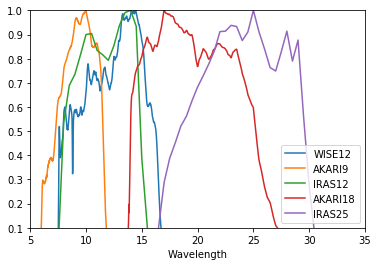
\includegraphics[width=150mm]{../Plots/RelSpectralResponse_MIR.png}
     \caption{Relative spectral response curves of the MIR bands used in this study, AKARI/IRC 9~$\mu$m, IRAS 12~$\mu$m, WISE 12~$\mu$m, AKARI 18~$\mu$m, and  IRAS 25~$\mu$m. AKARI/IRC 9~$\mu$m, IRAS 12~$\mu$m, WISE 12~$\mu$m bands are dominated by PAH emission (see Figure \ref{fig:inband_ionfrac_bar}. The AKARI 18~$\mu$m, and  IRAS 25~$\mu$m bands contain minimal PAH emission. }
     \end{figure*}


     \begin{figure*}
     \label{fig:inband_ionfrac_ratios}
     \centering
     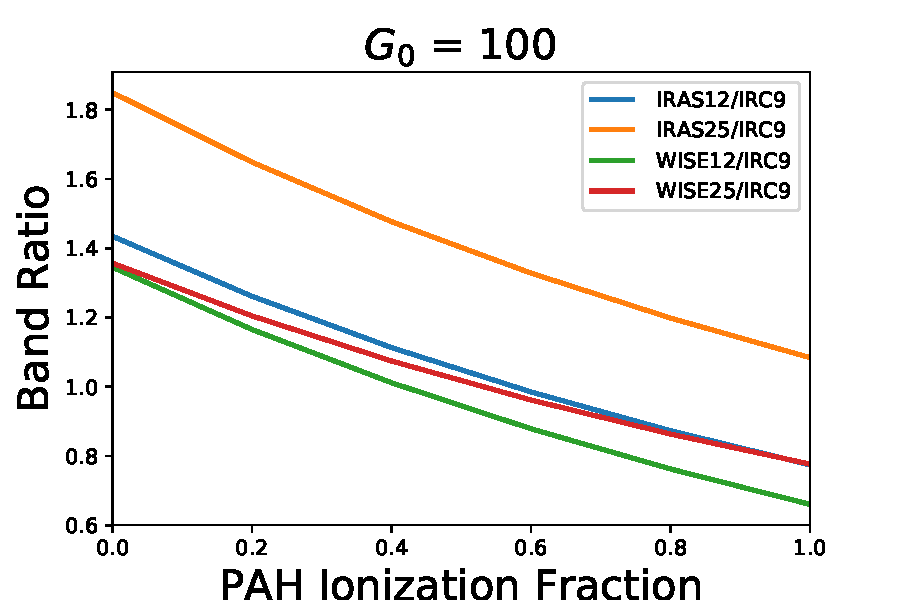
\includegraphics[width=80mm]{../Plots/band-ratio-G100.pdf}
     
\includegraphics[width=80mm]{../Plots/band-ratio-G1000.pdf}
     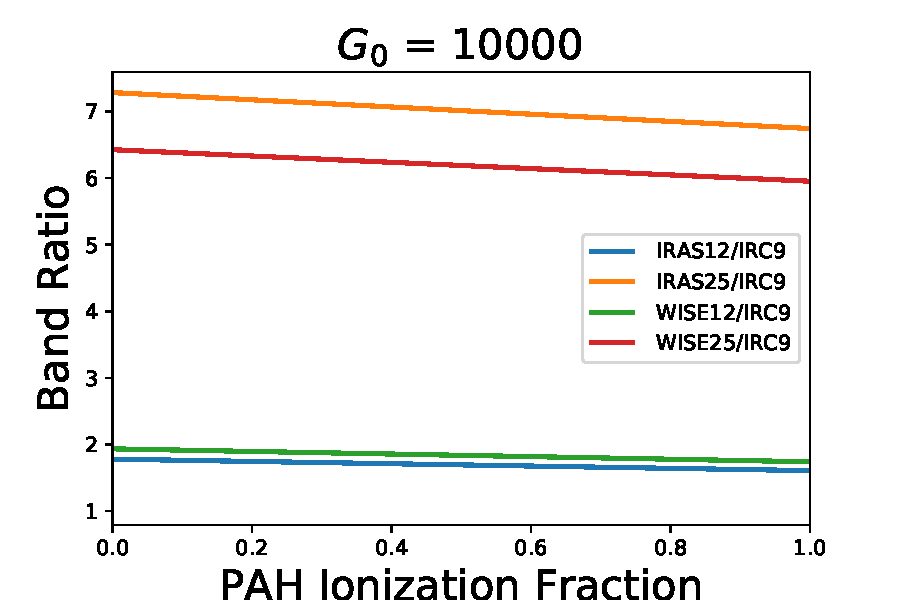
\includegraphics[width=80mm]{../Plots/band-ratio-G10000.pdf}
     \caption{For three ISRF strengths, $G_{0} = 100$, $G_{0} = 1000$, and $G_{0} = 10000$, the ionization fraction of PAHs vs. band ratios of IRAS12 and 25, and WISE 12 and 25 micron bads vs. the AKARI 9 micron band.  }
     \end{figure*}


     \begin{figure*}
     \label{fig:inband_ionfrac_bar}
     \centering
     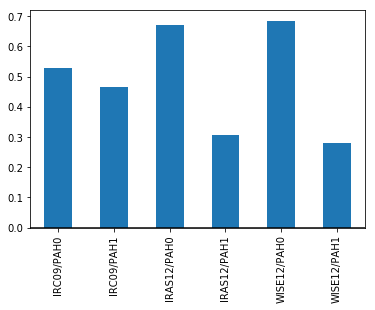
\includegraphics[width=150mm]{../Plots/InBandContribution_PAH_bar.png}
     \caption{Fractional contribution of ionized vs. neutral PAH emission, based on the DL01 dust SED model at $G_{0}$ of 1. $G_{0}$ is the interstellar radiation field strength relative to that of the solar neighborhood. PAH0 and PAH1 refer to neutral and ionized PAHs. }
     \end{figure*}



      We utilize the most recent version of the IRC data (Ishihara, et al., in prep.) This version has had an updated model of the Zodiacal light, fitted and subtracted. The details of the improved Zodi-model, which offers an improvement over that used for the IRAS all-sky maps, are given in \cite{kondo16}.
\begin{table*}
  \label{tab:data}
  \caption{Observational data sources used in this article}
  \centering
    \begin{tabular}{lrrrrr}
    \hline\hline
    %\tabletypesize{\scriptsize}
    %\tablecaption{Observational data sources used in this thesis\label{Data Sources}}
    Instrument & Central Wavelength & FWHM & Uncertainty & Reference \\
    \hline
    AKARI/IRC & 9~$\mu$m  &  \~{}10$"$ & \textless 10\%   & \citep{ishihara10} \\
    AKARI/IRC & 18~$\mu$m & \~{}10$"$  & \textless 10\%     & '' \\
    AKARI/FIS & 65~$\mu$m  & 63$"$ & \textless 10\% & \citep{doi15,takita16} \\
    AKARI/FIS & 90~$\mu$m  & 78$"$ & \textless 10\%   & '' \\
    AKARI/FIS & 140~$\mu$m & 88$"$ & \textless 10\%   & '' \\
    AKARI/FIS & 160~$\mu$m & 88$"$ & \textless 10\%   & '' \\
    COBE/DIRBE & 12~$\mu$m & & & \\
    COBE/DIRBE & 25~$\mu$m & & & \\
    COBE/DIRBE & 60~$\mu$m & & & \\
    COBE/DIRBE & 100~$\mu$m & & & \\
    IRAS/IRIS & 12~$\mu$m   & 4.0$'$ &   \textless 5.1\%       & \citep{iris05} \\
    IRAS/IRIS & 25~$\mu$m   & 4.0$'$ &    \textless 15.1\%      & ''\\
    IRAS/IRIS & 60~$\mu$m   & 4.2$'$ &    \textless 10.4\%      & '' \\
    IRAS/IRIS & 100~$\mu$m  & 4.5$'$ &   \textless 13.5\%       & '' \\
    Planck/HFI & 345~$\mu$m & 4.7$'$ & & \citep{hfi14viii} \\
    Planck/HFI & 550~$\mu$m & 4.3$'$& & '' \\
    WISE & 12~$\mu$m & & & &  \\
    \hline
    %% Text for table notes should follow after the \enddata but before
    %% the \end{deluxetable}. Make sure there is at least one \tablenotemark
    %% in the table for each \tablenotetext.
    %\label{TabData}
  \end{tabular}
\end{table*}

    The AKARI Far Infrared Surveyor (FIS) gives us photometric data around the peak of the typical thermal dust SED. FIS was equipped with four wavebands: two narrow bands centered at 65~$\mu$m and at 160~$\mu$m, and two wide bands at 90~$\mu$m and at 140~$\mu$m. An all-sky survey was carried out at each band \citep{kawada07}, and the processed maps have been publicly released \citep{doi15}.

     The Planck Space Observatory (Planck) High Frequency Instrument (HFI) all-sky maps, spanning 100 to 857~GHz \citep{hfi14viii} constrain the far IR dust emissivity. This study utilizes the 857~GHz (345~$\mu$m) and 545~GHz (550~$\mu$m) bands.

     Data from the Infrared Astronomical Satellite \citep{iras84} all-sky surveys are used to supplement the similarly-centered AKARI photometric bands. The IRAS 12~$\mu$m band is similar to the AKARI 9~$\mu$m band in terms of the sky coverage, central wavelength, and especially in that both surveys are heavily dominated by zodiacal light. We use the Improved Reprocessing of the IRAS Surveys (IRIS) \citep{iris05}, which use undergone a zodiacal-light removal. The Zodiacal light model, however differs between the two bands. The IRAS Zodi-subtraction is primarily based on the \cite{kelsall98} model.

\subsection{AME Data}
     We utilize the AME component separation map, from the Planck Collaboration's Public Data Release 2. Details of the foreground contribution estimates are given in \cite{planckXII}. We caution readers that this AME map was created primarily for the purpose of isolating the CMB from galactic microwave emission. It is not to be taken as a perfect isolation of the AME. We employ it in this work, simply because there is no other all-sky AME estimate available. We also quote AME estimates for 98 circular apertures, found in \cite{planckXV}, that were made using a more careful region-by-region component separation method at 1-degree resolution.

\subsection{All-sky Data Processing}

      The HFI, FIS, and IRIS maps used here are downloaded from their respective online repositories, as all-sky HEALPix \citep{gorski15} NSIDE 2048 maps. In the case of the IRC maps, we first create HEALPix maps from the 4,857 all-sky survey tiles using the Aladin all-sky data visualization platform \citep{bonnarel00}. NSIDE 2048 implies an average pixel spacing of 1.7$'$. The maps are then degraded to NSIDE 1024 before carrying out the Gaussian-beam smoothing to a 1-degree FWHM. Following the smoothing process, the maps are degraded once more to NSIDE 256. The value of each of the larger NSIDE 256 pixels, comes from the mean of its parent NSIDE 1024 pixels. The purpose of this processing is to ensure that all of the maps have the same resolution as the PR2 AME map.


\section{Analysis}
\label{sec:analysis}

The analysis we have done so far is done from 3 perspectives, but with all 3 relying on 1-degree resolution, Planck-based AME data. We start from a widely-cast net: an AME to IR comparison on an all-sky basis, looking at trends among, essentially, all pixels in the all-sky maps except for those within 10 degrees of the ecliptic plane. Then we move to a slightly more regionalized comparison, looking at the set of AME-prominent galactic clouds identified by the \cite{planckXV} (wherein we keep our analysis parallel to theirs, to maintain comparability between their IRAS-Planck based result, and our result which adds-in AKARI data and dust SED fitting.) Lastly, we highlight a particular AME-dominated region, the ``Meissa ring'', otherwise known as the $\lambda$ Orionis molecular ring \citep{maddalena86,maddalena87}. Our motivation is to highlight the limitations of low resolution AME data, at 3 different scales, and help to promote higher resolution, more localized, structural studies of AME and spinning dust.

\subsection{All-sky Pixel Domain Analysis}

	In order to look more closely at the variations between the individual bands' maps, we also include a pixel-by-pixel analysis. Figure \ref{fig:AMEvsDust_allsky_allbands} shows the result of such a comparison, for each of the 19 bands sampled. The AME data comes from the AME component map provided in the Planck Public Release 2, produced by the COMMANDER component separation method.

    To keep our analysis comparable to previous works, we carry-out the analysis by excluding pixels within 10 degrees of the ecliptic plane, where the Zodi-residuals can be a problem (especially in the MIR.) The remaining pixels are divided into ``high galactic latitudes'' (more than 10 degrees from the galactic plane), and ``low to mid galactic latitudes'' (within 10 degrees of the plane).
    %While it is true that the story of pixels close to the plane tends to be complicated, it is also true that at high galactic latitudes, where IR dust emission is fainter, Zodi-subtraction uncertainties become more significant.

    We can quickly see that, for all of the bands, there is a first-order correlation between the IR with the AME. Figure \ref{fig:AME_IR_crosscorr_allbandsg} visualizes the cross-correlation matrix for each of the IR bands and the AME for both the Pearson-based and Spearman-based cross-correlation matrices. With either test, the AME does not show a strong correlation with other bands at high latitudes. At lower latitudes, the FIR bands show stronger correlation for the Pearson test, but there appears to be an even correlation across all bands in the case of the Spearman rank test. The AKARI 9 micron bands, and the other PAH-tracing bands show a stronger correlation only relative to the bands from 18 to 60 microns. The WISE 12 micron band is show for comparison purposes, but the version of the WISE 12 micron map used here has been produced only for visualization purposes and is not yet vetted for scientific analysis.

    Even excluding pixels near the ecliptic plane, and separating the sky into two GLAT ranges, the situation is very difficult to interpret. To understand if the same pattern persists across the sky rather than presenting only for the all-sky average, we repeat the correlation analysis for GLAT bins. For each degree of galactic latitude, we cross correlate that Planck modified blackbody fitting results vs. the AME and the AKARI 9 micron intensity. (This comes with the caveat that the galactic plane is much more heavily sampled than the galactic poles.) Figure \ref{fig:PlanckModBBvsAMEandA9_byGLAT} shows the results.


      \begin{figure*}
        \label{fig:AME_IR_crosscorr_allbandsg}
        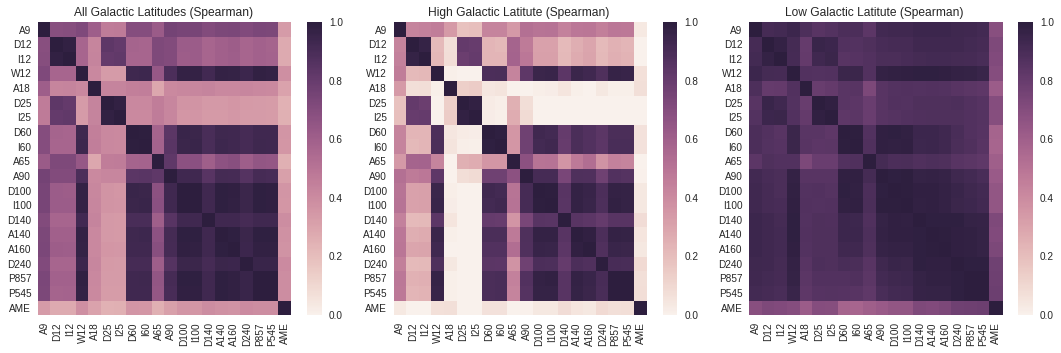
\includegraphics[width=185mm]{../Plots/all_bands_corr_matrix_wAME_spearman.png}
        \centering
        \caption{A colorized visualization of the ALL-SKY cross-correlation matrix for the 19 infrared bands sampled and the AME map. These results are based on the full sky (but omitting pixels within 10 degrees of the ecliptic plane) cross correlation of each band vs. every other band and the AME map. Plots on the top row are based on the Spearman rank correlation test. Those on the bottom are based on the Pearson correlation coefficients. }
      \end{figure*}



      \begin{figure*}
        \label{fig:AMEvsDust_allsky_allbands}
        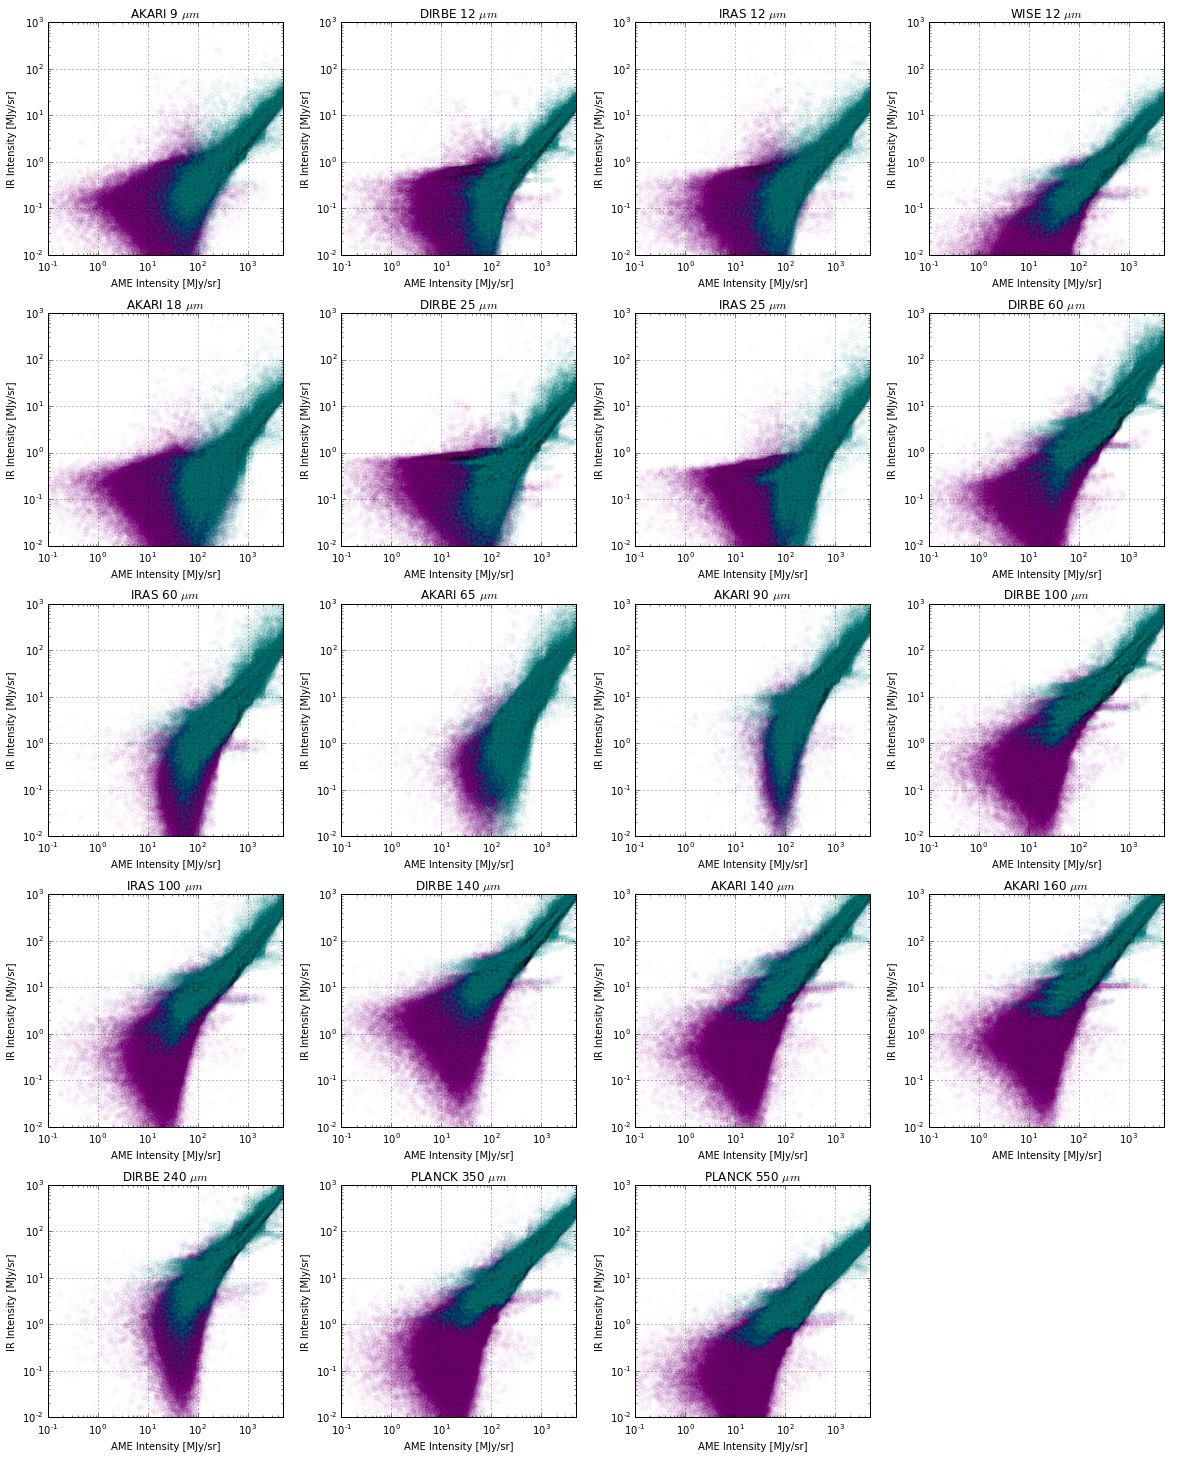
\includegraphics[width=145mm]{../Plots/AMEvsDust_allsky_allbands.png}
        \centering
        \caption{ALL-SKY plots of each of the 19 infrared bands' photometry results against those of the AME map. Similar to plots from the previous section, however these are produced on an all-sky basis. Cyan points represent pixels within 5 degrees of the galactic plane. Magenta points are pixels over 5 degrees from the galactic plane. Pixels within 5 degrees of the ecliptic plane are not plotted. Due to the large number of pixels plotted, a low alpha value is used (0.02). This helps to visualize the bulk of the pixels, but also means that portions of the plot with low point-density may seem blank on the page. Figure \ref{fig:AME_IR_crosscorr_allbandsg} shows the cross-correlation test results.}
      \end{figure*}


      \begin{figure*}
        \label{fig:PlanckModBBvsAMEandA9}
        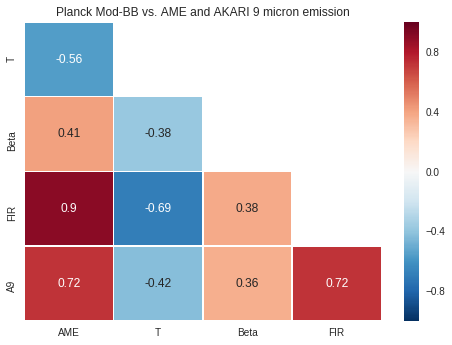
\includegraphics[width=185mm]{../Plots/PlanckModBBvsAMEandA9.png}
        \centering
        \caption{A cross-correlation test (Spearman) of AME vs. dust radiance (R), temperature (T),  emissivity index (Beta), and the AKARI 9 micron brightness (A9), of the whole sky. Thermal dust parameters are provided in the Planck Coll. PR2 data. This provides a simplified picture of the AME vs. IR dust emission relationship. We can see that the results are consistent with the cross-correlation of AME vs. the 19 photometric intensities in Figure \ref{fig:AME_IR_crosscorr_allbandsg}. This plot gives the results using the whole sky. Figure \ref{fig:PlanckModBBvsAMEandA9_byGLAT} shows correlation results broken down into 1-degree GLAT bins.}
      \end{figure*}

      \begin{figure*}
        \label{fig:PlanckModBBvsAMEandA9_byGLAT}
        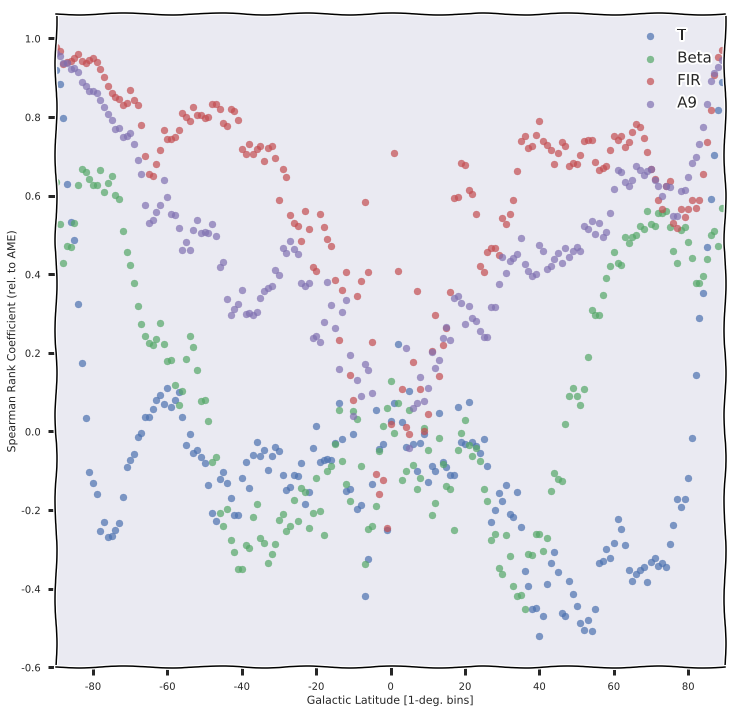
\includegraphics[width=90mm]{../Plots/PlanckModBBvsAMEandA9_byGLAT.png}
        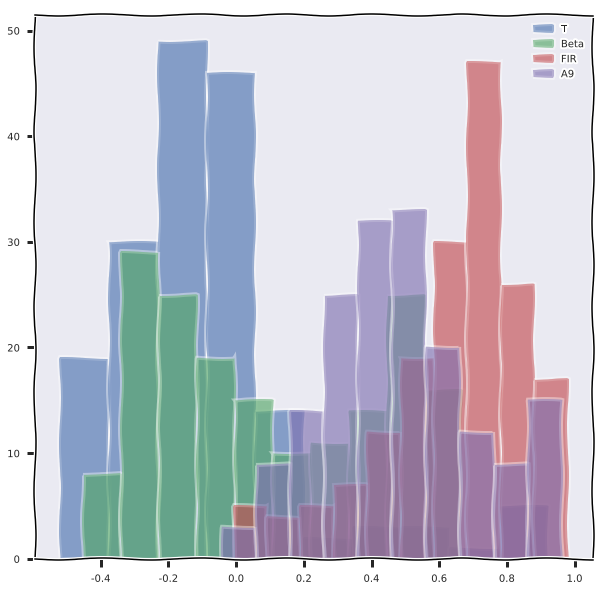
\includegraphics[width=90mm]{../Plots/PlanckModBBvsAMEandA9_hist.png}
        \centering
        \caption{A cross-correlation tests (Spearman) of AME vs. dust radiance (R), temperature (T),  emissivity index (Beta), and the AKARI 9 micron brightness (A9), by GLAT. The order of strongest to weakest correlation basically remains constant from pole to pole. (Except near the galactic plane, and around GLAT 40  }
      \end{figure*}


\subsection{Analysis of Planck Collaboration AME Candidate Regions}

     Previously, \cite{planckXV} (hereafter, PCXV) had identified and analyzed a list of regions where the AME appeared to stand out, relative to estimates of known microwave foregrounds. The full set includes 98 regions. While the majority of these regions showed only low significance AME, or a high potential contribution from free-free emission, 27 of showed highly significant AME. We re-examined the full set of 98 regions, employing data from 19 photometric bands, from the AKARI, Planck, IRAS, and WISE data sets. The major goals are 1) To see how the AME to IR comparison looks with the AKARI data, and 2) To apply a dust SED fitting analysis to these regions. While tackling these goals, we attempted to keep our analysis is comparable as possible to the PCXV analysis by following their circular aperture photometry scheme. The process can be summarize as follows:

     1) For each region, the total flux within a 1 degree radius circular aperture is summed.

     2) A background annulus, with inner radius 80$'$ and outer radius 100$'$, is placed around the source aperture. The median value of pixels inside the annulus is taken, and then scaled up to solid angle of the central source aperture. This is used as background level, to be subtracted from the source flux.

     3) The noise level is estimated from the standard deviation of the background annulus pixels (estimating the noise level of large regions such as these is not a straightforward task.) We should note that for a few regions, the photometry done here using the PR2 map, and the photometry done on the same regions in PCXV, show discrepancies in the total flux measured (see Figure \ref{fig:AME_PCXVvsPR2}). These discrepancies do not alter our conclusions.

     Once photometry results were gathered for all of the 98 regions, we then performed a full dust SED fitting,

    The SED of the different fields were fit using the \cite{galliano11} dust model. We used the amorphous carbon and silicate dust mixture. Indeed, this dust mixture is more emissive than the standard silicate-graphite \citep{draine07}, by a factor of 2-3. As was shown by Herschel, in the LMC \citep{galliano11}, and by Planck, in the Milky Way \citep{planck16}, this increase of emissivity is necessary to have a proper fit of the sub-mm emission. We assume that the radiation field heating this dust mixture is the Galactic ISRF \citep{math83}, scaled by a factor $U$. We also assume, following \cite{dale01}, that the dust is exposed to a distribution of starlight intensity, distributed as:

    \begin{equation}
        \label{eq:U}
          dM_{dust}\propto{} U^{-\alpha}dU
     \end{equation}

    between $U_{min}$ and $U_{max}$, where $U_{min}$, $U_{max}$ and $\alpha{}$ are free parameters. An old stellar population template (PEGASE; \citep{fioc97}) is added to this SED in order to model the near-IR emission. The emission of this dust model is demonstrated in Fig. \ref{fig:galliano11_templates}. We perform, for the moment, a simple least-squares analysis. The results of the SED fitting vs. the AME are shown in Figure \ref{fig:AME_regs_J13}. For the vast majority of the samples, the fits are reasonable, with the $\chi{}^{2}$ distribution (see Fig. \ref{fig:AME_PCXVvsPR2}) appearing as we expect.

\begin{figure*}
  \label{fig:galliano11_templates}
  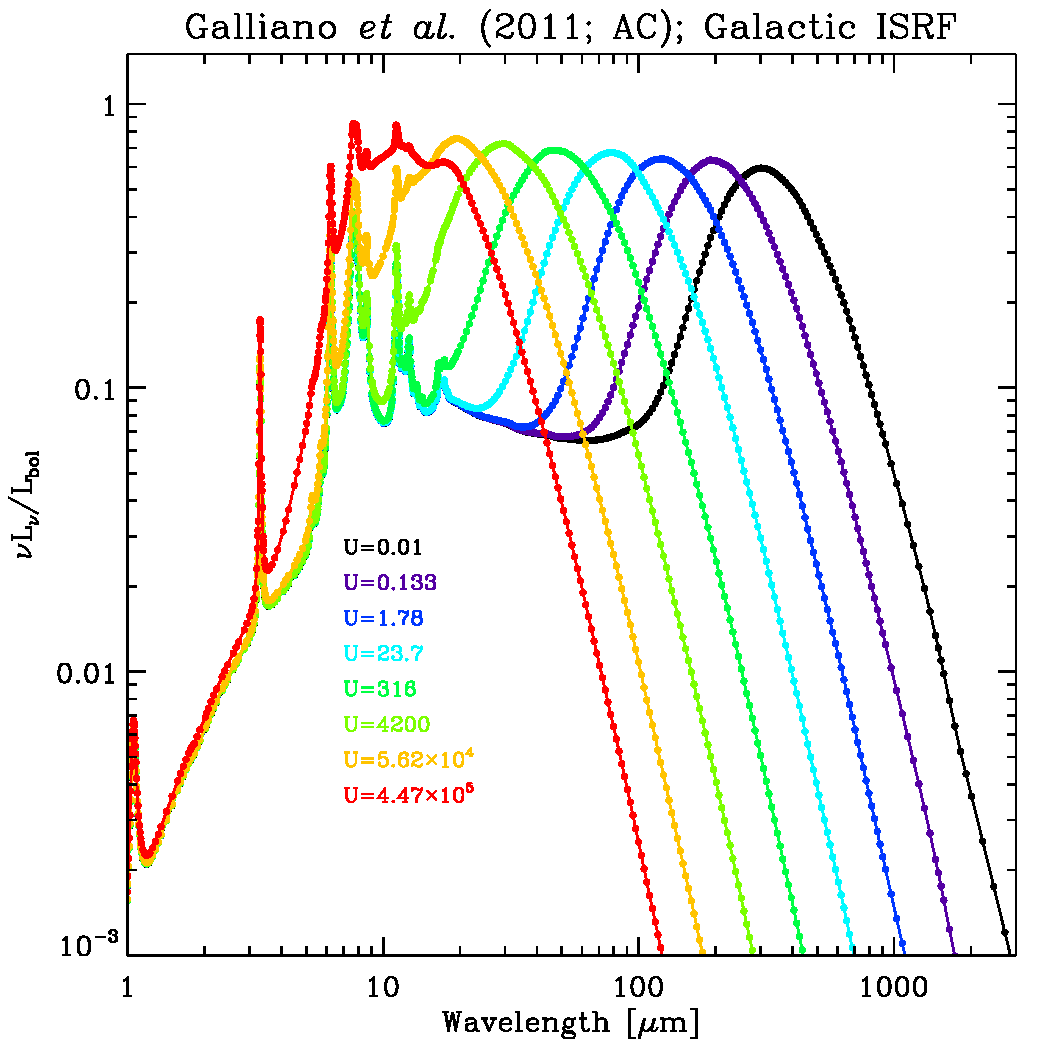
\includegraphics[width=80mm]{../Plots/template_deltaU_G11_AC.pdf}
  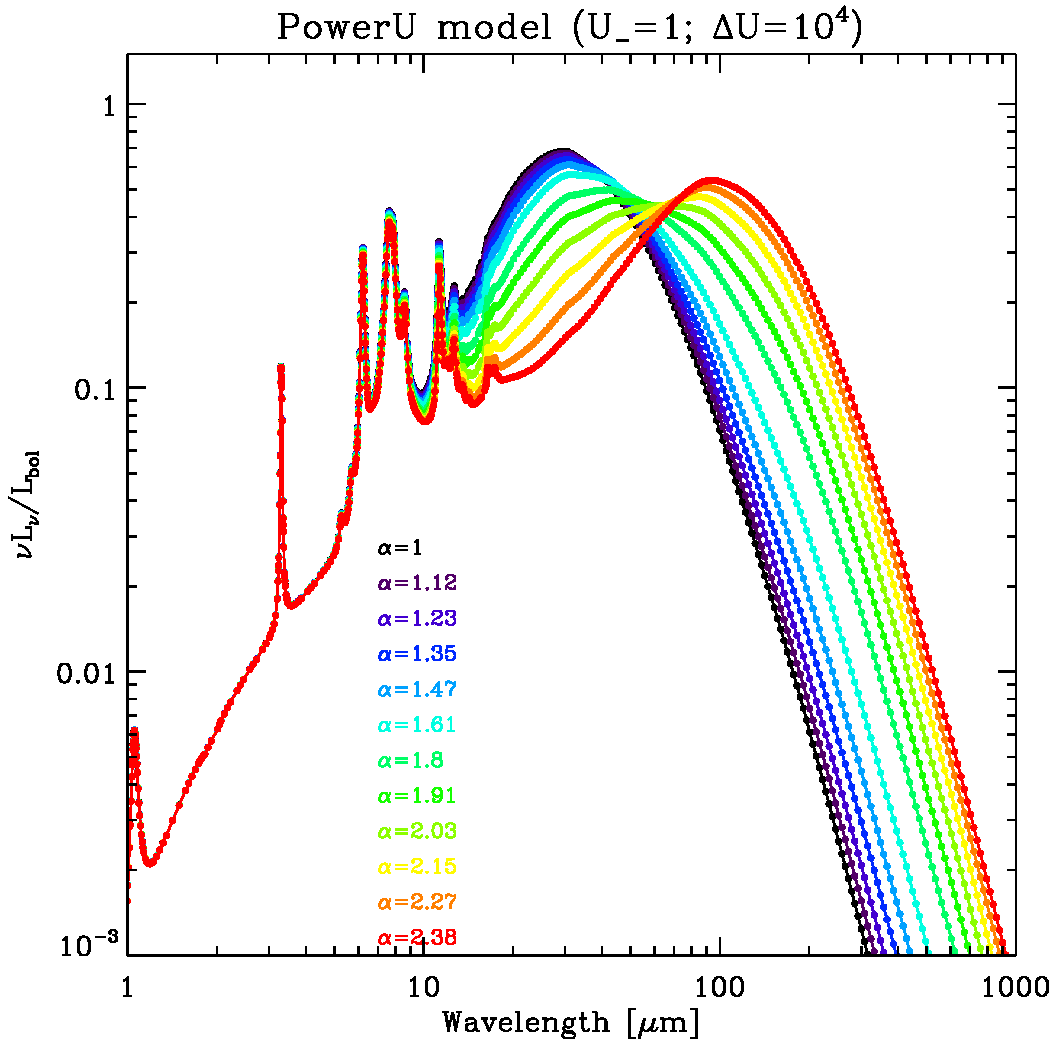
\includegraphics[width=80mm]{../Plots/template_powerU_alpha_G11_AC.pdf}
  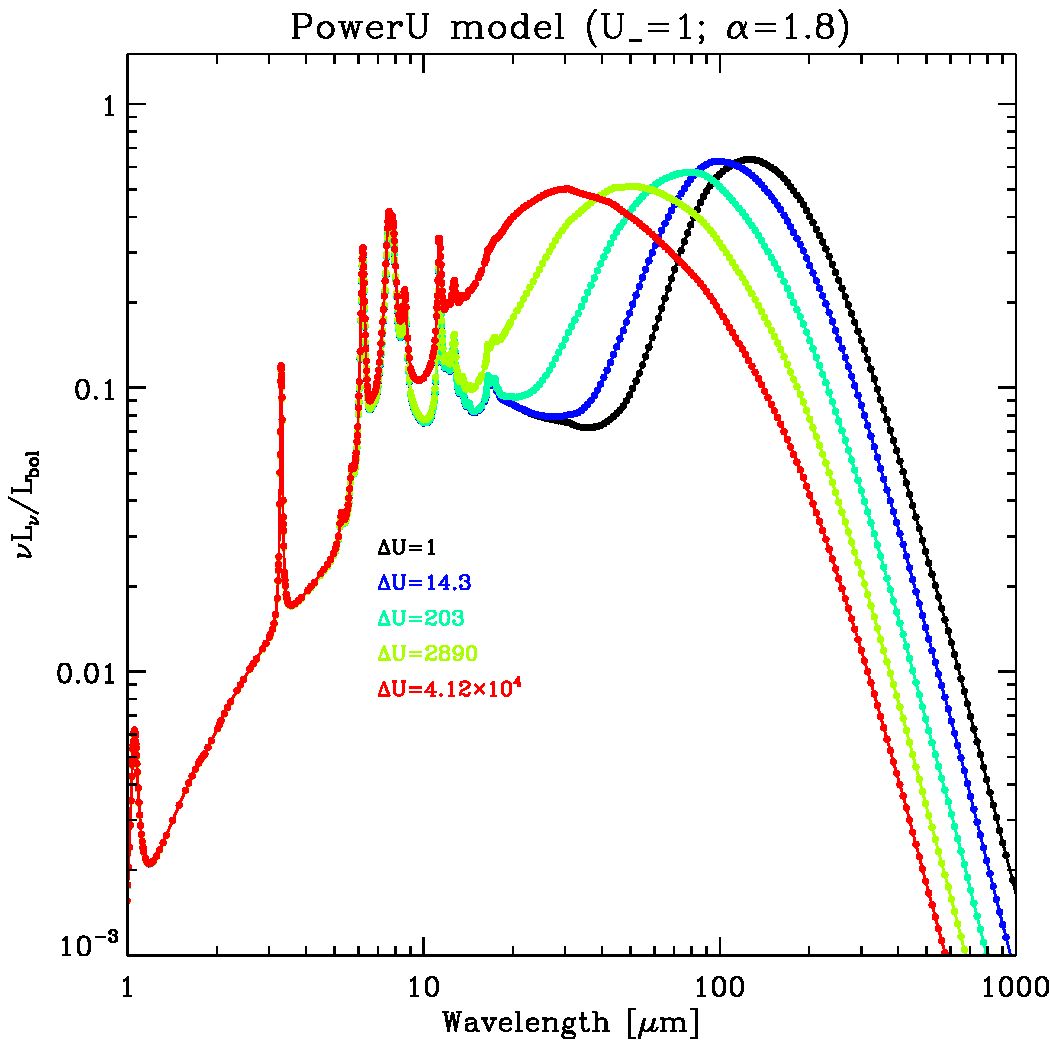
\includegraphics[width=80mm]{../Plots/template_powerU_DU_G11_AC.pdf}
  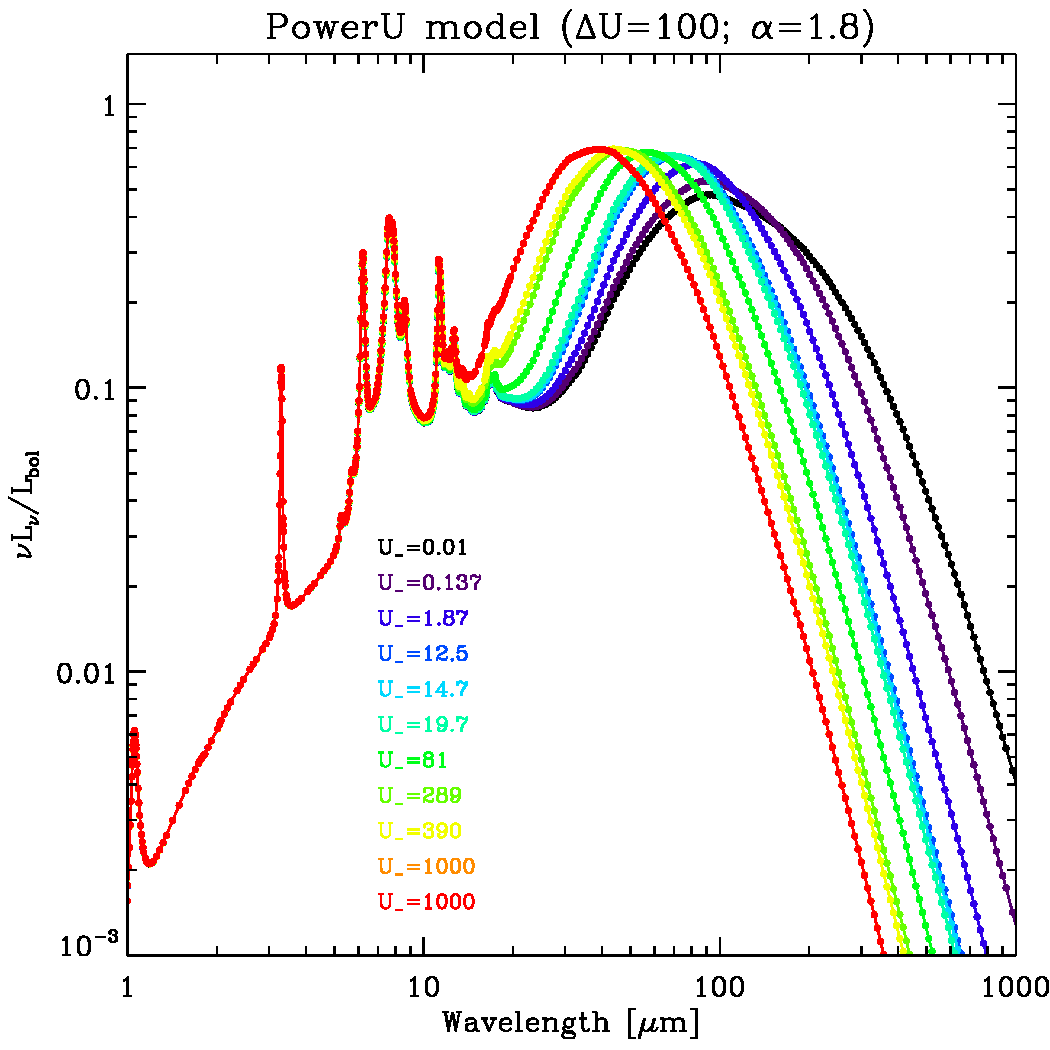
\includegraphics[width=80mm]{../Plots/template_powerU_Um_G11_AC.pdf}
  \centering
  \caption{Dust templates of \cite{galliano11}. The upper-left panel shows the variation of a uniformly illuminated mixture, as a function $U$. The other three panels show the variations of the emission of a dust mixture exposed to a distribution of starlight intensity, varying each parameter of Eq. \ref{eq:U}.  }
\end{figure*}

     Two comparisons are shown - AME vs. PAH mass and AME vs. total dust mass, for two different AME data sets. The AME (PR2) data indicates the results of this work (our own photometry on the publicly available Planck 'COMMANDER' algorithm based AME map.) The AME (PCXV) plots, on the bottom, indicate that the AME flux values are those quoted from the PCXV analysis (wherein component separation, of AME from known foregrounds, was done region-by-region.) Furthermore, the regions themselves are categorized as high (red circles) or low (blue circles) significance AME. Simply based on Figure \ref{fig:AME_regs_J13}, it is difficult to discern a difference on the correlation strengths. To statistically evaluate the situation, we employ the Bootstrap re-sampling approach, first introduced by \cite{efron79}. This involves creating 100,000 random re-sampled sets of the data. We use the "with replacement" approach, meaning that a data point may be selected multiple times in a single re-sampling iteration. However the size of the re-sampled set is the same is the input set size. For each random set we run a correlation test, resulting in a distribution of correlation coefficients. The results of the Bootstrap analysis are given in Figure \ref{fig:AME_boostrap_mass_regs_all}. The distributions of correlation coefficients for AME vs. PAH mass, and AME vs. total dust mass., appear to be distinct. Mean correlation coefficients are separated by 0.1+/-0.05-0.07.

%     If anything, the correlation tests indicate that the regions most reliably identified as AME-prominent, had a weaker correlation with both dust mass and with PAH mass. However, here we must be very cautious, considering the lower sample size of highly significant AME regions. Moreover, the difficulties in noise estimates, and the inherent uncertainty in the AME component separation process.

\begin{figure*}
  \label{fig:AME_regs_J13}
  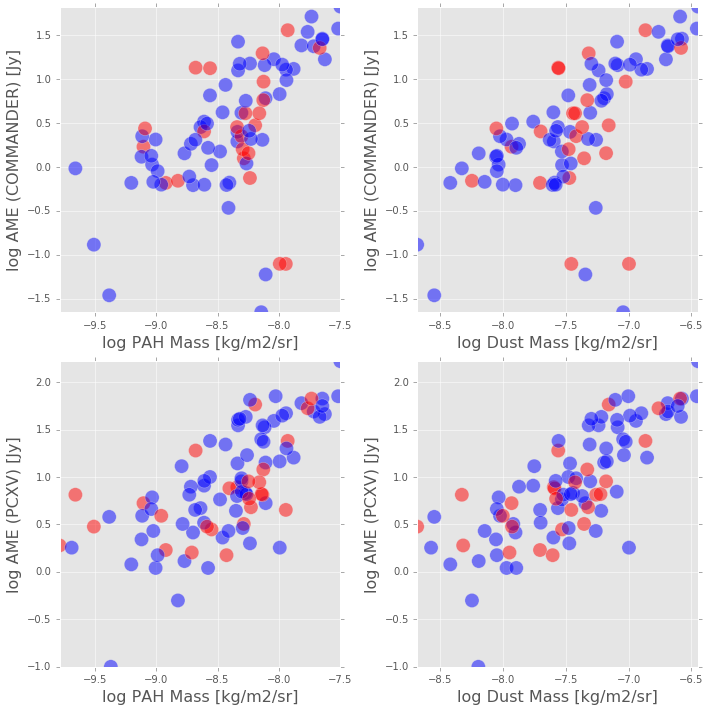
\includegraphics[width=150mm]{../Plots/AMEvsDust_regs_J13.png}
  \centering
  \caption{Results of circular aperture photometry and dust SED fitting for 98 regions listed in PCXV. Red dots indicated regions with significant AME. Blue dots indicated regions with low/zero significance AME. }
\end{figure*}

\begin{figure*}
  \label{fig:AME_PCXVvsPR2}
  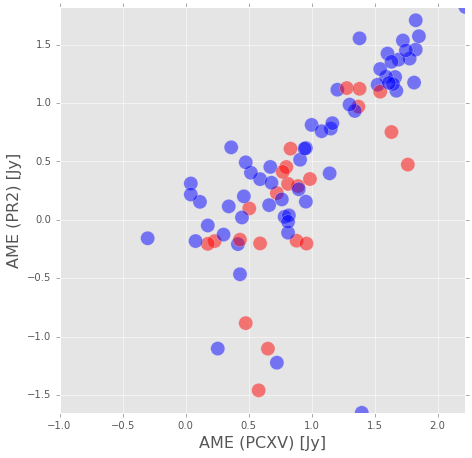
\includegraphics[width=80mm]{../Plots/PCXVvsPR2.png}
  \centering
  \caption[width=75mm]{Left: Cross-comparison of the PCXV photometry results and the results of this work, based on the Planck Collaboration PR2 AME map.}
\end{figure*}

\begin{figure*}
  \label{fig:AME_regs_chi2}
  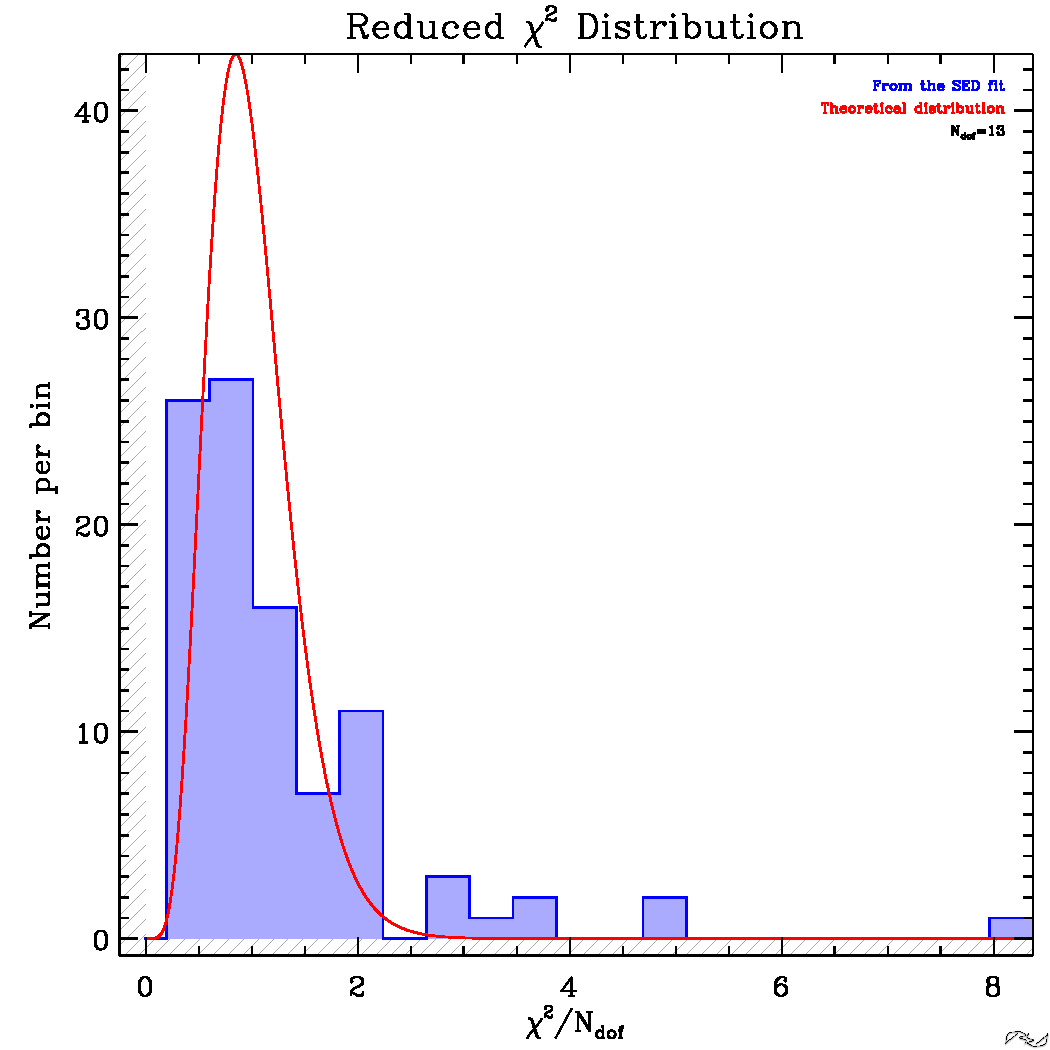
\includegraphics[width=75mm]{../Plots/histo_chi2red.pdf}
  \centering
  \caption{Histogram showing the $\chi^{2}$ distribution of the dust SED itting, to the AME region apertures. }
\end{figure*}

\begin{figure*}
  \label{fig:AME_boostrap_mass_regs_all}
  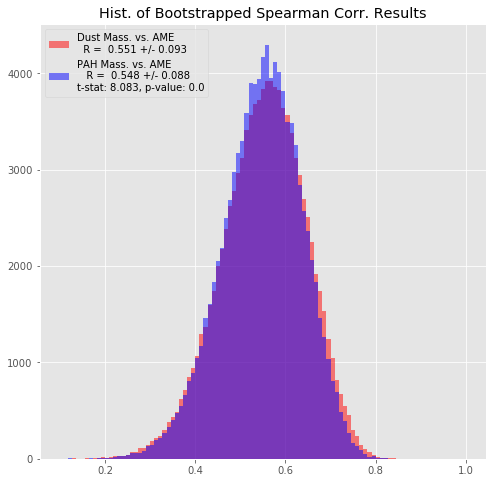
\includegraphics[width=80mm]{../Plots/AMEregs_bootstrap_mass_spearman_PR2.png}
  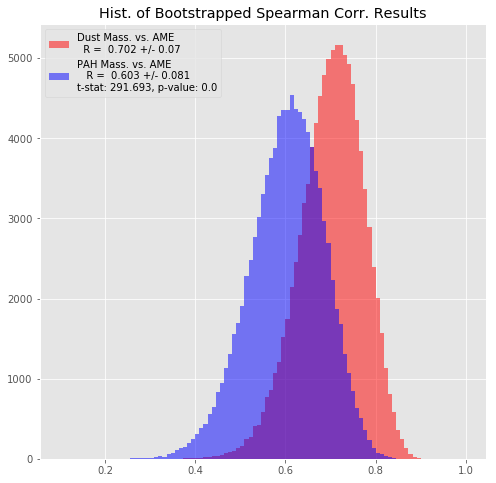
\includegraphics[width=80mm]{../Plots/AMEregs_bootstrap_mass_spearman_PCXV.png}
  \centering
  \caption{Top Left: Histogram showing the distribution of Pearson correlation coefficient results (R), based on 100,000 Bootstrapped sub-samples for each of the two comparisons (AME vs. total dust mass and AME vs. PAH mass.), based on PCXV AME flux values of the full set of 98 candidate regions. Top right:  The same comparison, but using flux values obtained by directly performing circular aperture photometry on the Planck PR2 COMMANDER AME component map. Bottom left: PCXV bootstrap analysis using Spearman rank test. Bottom right: Spearman rank test for PR2 results. R values quoted for each comparison are that R-distribution's mean, and the error bars are the standard deviation. }
\end{figure*}

\begin{figure*}
  \label{fig:AME_boostrap_lum_regs_pr2}
  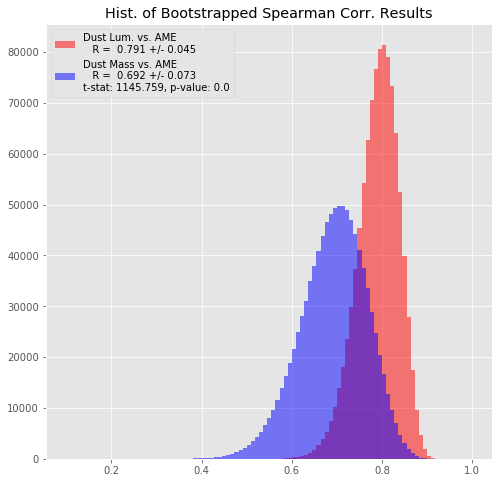
\includegraphics[width=80mm]{../Plots/AMEregs_bootstrap_DmassDlum_spearman_PCXV.png}
  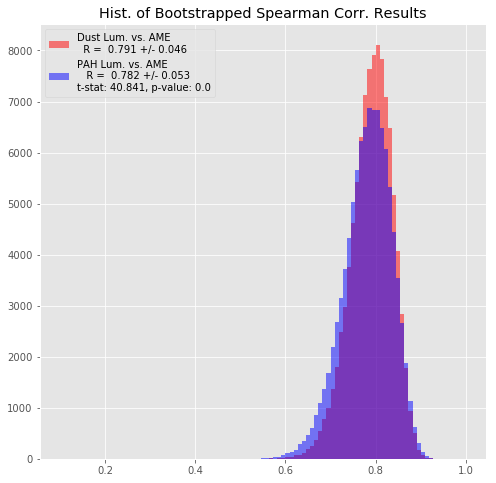
\includegraphics[width=80mm]{../Plots/AMEregs_bootstrap_PmassDlum_spearman_PR2.png}
  \centering
  \caption{The plots above use the same comparison method as in Figure \ref{fig:AME_boostrap_mass_regs_all}. However the dust fitting parameters being compared are }
\end{figure*}



\subsection{Analysis of the $\lambda$~Orionis Region}

	Having looked at the AME vs. dust emission story on a very course scale, we now introduce our analysis of a particular region. The $\lambda$~Orionis molecular ring, shown in Figure \ref{fig:orionis-akari9} as it appears in 1-degree smoothed AKARI 9~$\mu$m data, indicates excess microwave emission attributed to AME \citep{planck15XXV}. At approx. 10 degrees wide, we can see the outline of the structure even in the low (1 degree FWHM) resolution Planck-COMMANDER AME map. This is one of the only structures on the sky with a relatively well-distinguished shape at such low resolution. In order to shift towards an investigation of individual AME-prominent regions, we have carried out an initial comparison of the AME of this region with its mid to far-IR dust emission.

	Figure \ref{fig:orionis-img} shows how the region looks, for 12 different photometric bands, from the mid to far IR. The contours show the region's structure as given by the Planck PR2 AME map. Figure \ref{fig:orionis-corr} shows simple IR to AME cross correlation plots, for all pixels within the 10 by 10 degree $\lambda$~Orionis region. Our findings for lambda $\lambda$~Orionis indicate an AME-PAH correlation, but we are unable to argue for a causal link.

\begin{figure*}
  \label{fig:orionis-akari9}
  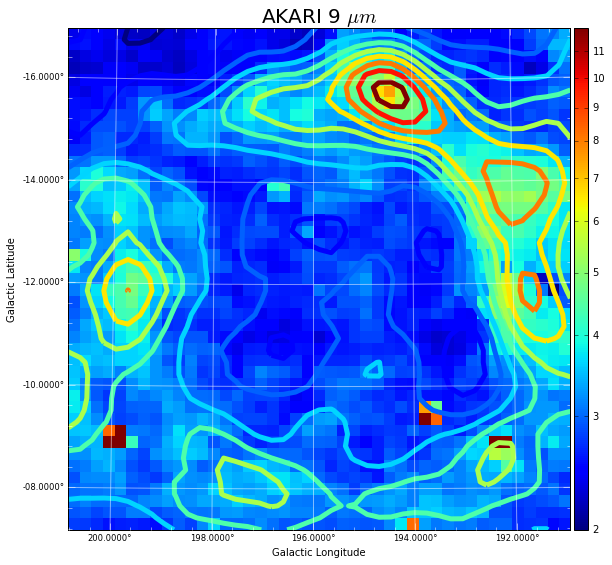
\includegraphics[width=150mm]{../Plots/lOrionis_AKARI9.png}
  \centering
  \caption{$\lambda$~Orionis as it appears in the AKARI 9~$\mu$m data. Contours indicate the AME, as given by the Planck PR2 AME map. The image is smoothed to a 1-degree PSF (much larger than the original 10 arcsec map. The $\lambda$~Orionis star itself is approximately located at the center of the image. The dust wave structure, described by *citation needed*, is apparent, and seems to coincide with a local maxima in the PR2 AME contours. The units are MJ/sr. )}
\end{figure*}

\begin{figure*}
  \label{fig:orionis-img}
  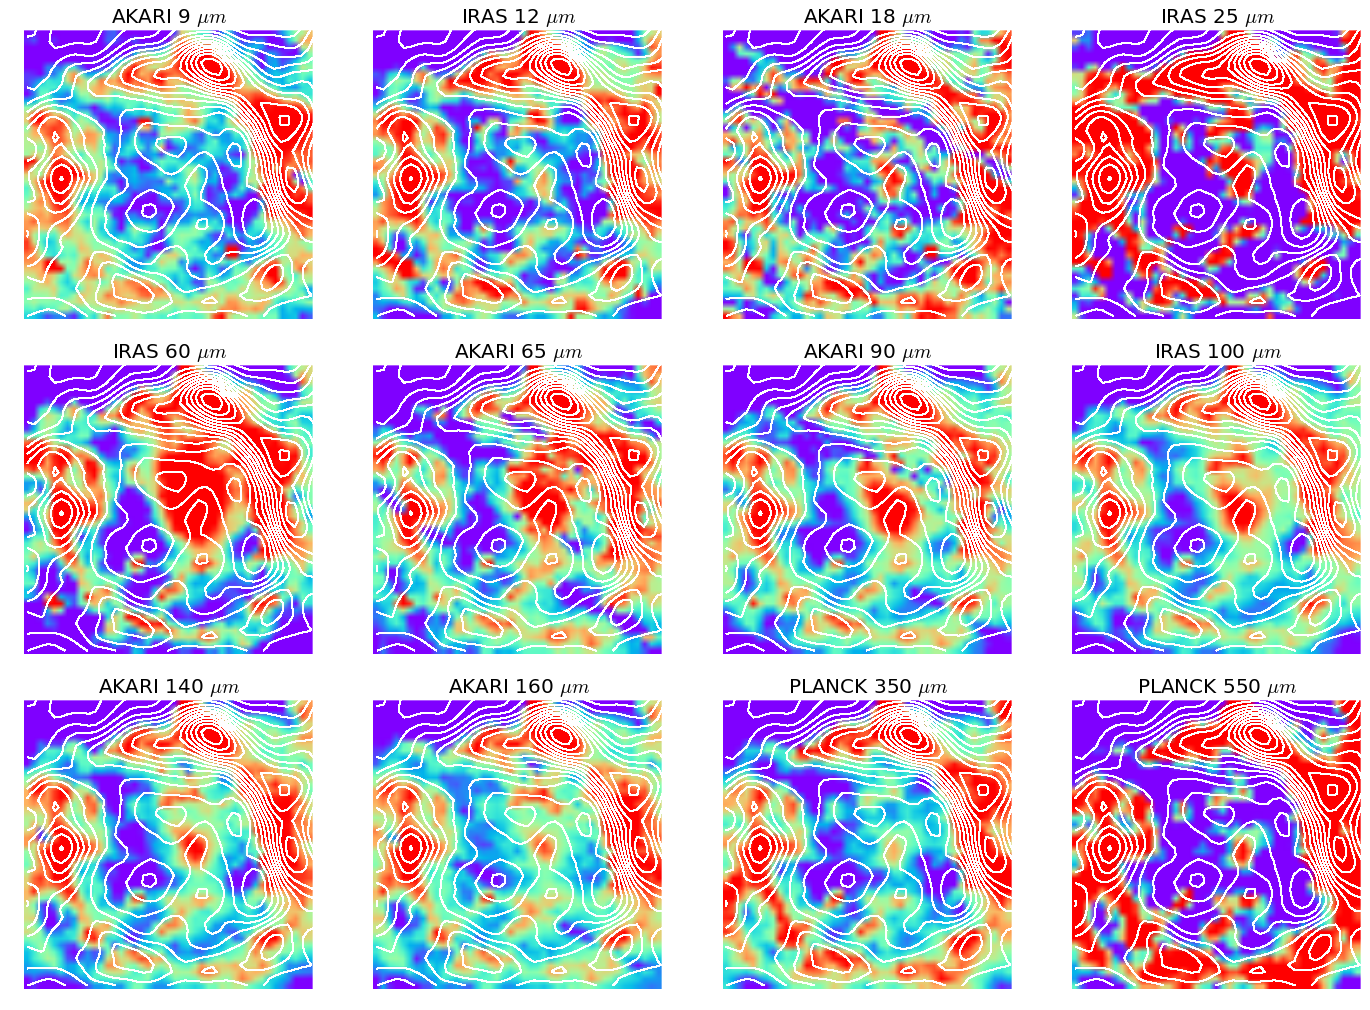
\includegraphics[width=170mm]{../Plots/lOrionis_grid_img.png}
  \centering
  \caption{A grid of thumbnails showing the $\lambda$~Orionis region's structure, at 12 wavelengths, along with AME contours (shown in white countours. Spatial correlation seems to be the best at the shortest and longest wavelengths (AKARI/IRC 9~$\mu$m and Planck/HFI 550 micron) .}
\end{figure*}

\begin{figure*}
  \label{fig:orionis-corr}
  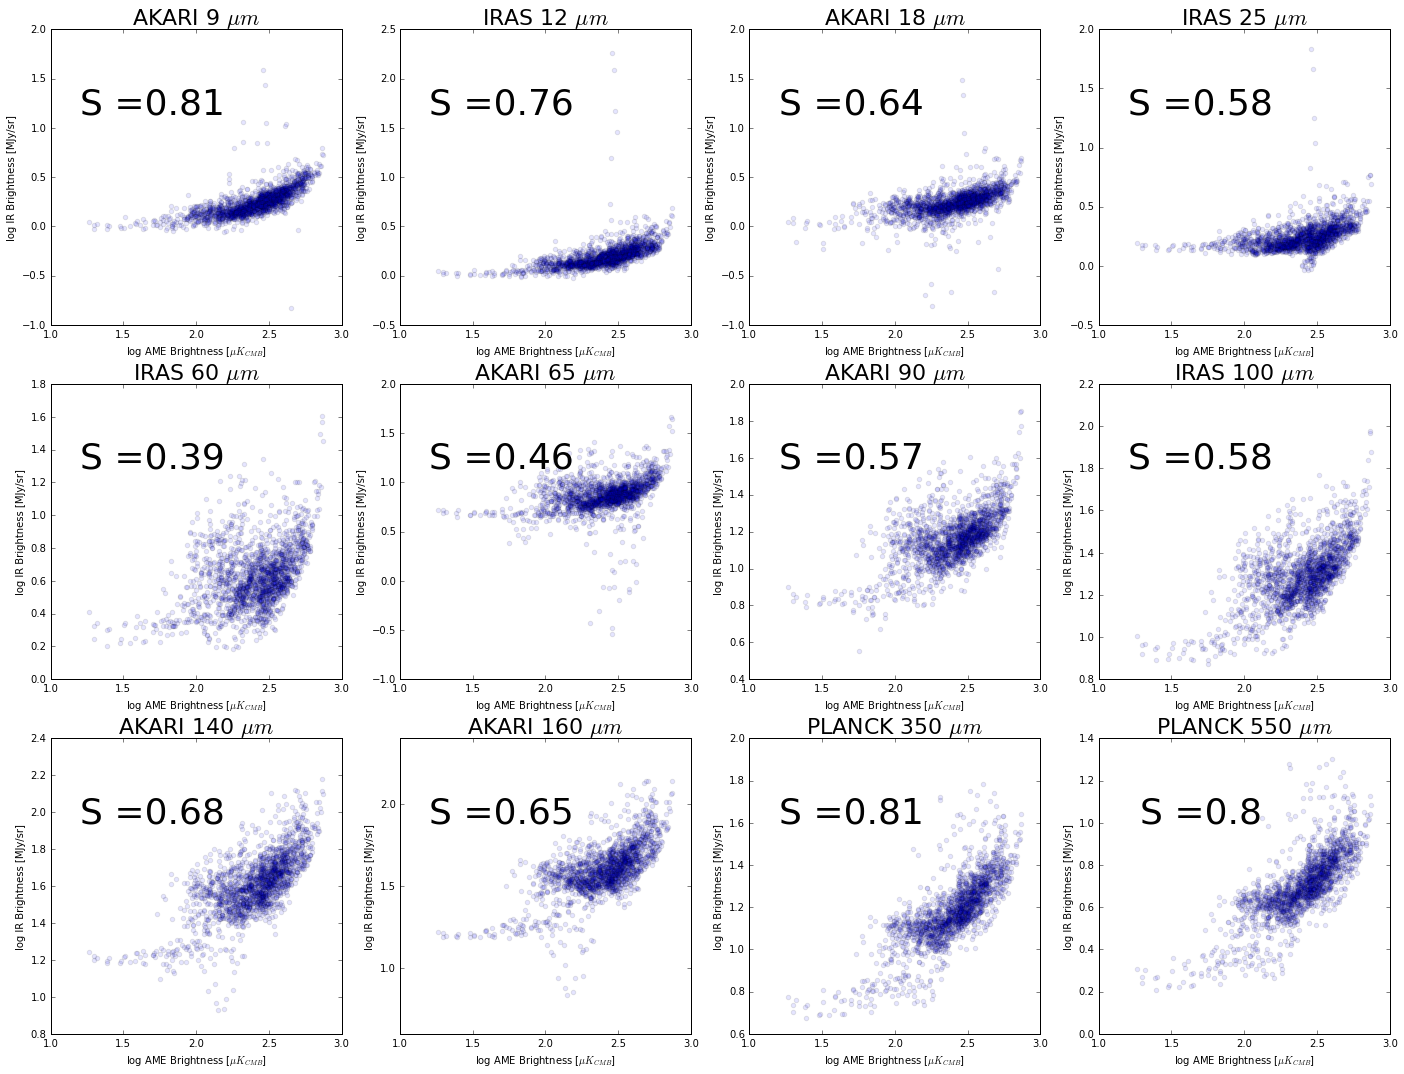
\includegraphics[width=170mm]{../Plots/orionis_correlations_AME.png}
  \centering
  \caption{Pixel cross-correlation for all pixels in the $\lambda$~Orionis cut-out region.  $S$ indicates the Spearman rank correlation coefficient for each plot.}
\end{figure*}

\section{Discussion}
  \label{sec:discussion}


      \subsection{AME:Dust}

        As noted in Section 1, previous studies found that the AME generally correlates at dust-related IR wavelengths \citep{ysard10b,planckXV, hensley16}. We see the same overall pattern in the present study, for each of the three scales examined: the all-sky pixel-based analysis, the re-examination of Planck AME Candidate regions, and the inspection of the $\lambda$~Orionis region.

         In our all-sky, pixel-by-pixel comparison, we find that all of the 19 wavelengths sampled show a first-order correlation with the AME. This is again consistent with the previous investigations of the AME cited above, wherein the only differences found are minor. Without applying further dust SED fitting, this analysis seems to concur with \cite{hensley16} in that the FIR bands (in their work, they used the dust radiance) show the tightest correlation. In \cite{hensley16}, the galactic plane is masked, whereas we mask only the pixels which have missing data from any of the 19 maps, as well as pixels within 10 degrees of the ecliptic plane (due to residual zodiacal light emission in the MIR maps.)

        In the case of the AME candidate regions, do we find evidence of a statistically stronger relationship between AME and total dust mass than AME vs. PAH mass, for the full set of 98 regions. We were able to confirm that the correlation coefficients are statistically distinct, via boostrap re-sampling (with replacement.) However the difference is marginal. Moreover the full set of 98 regions includes many regions that are either near the galactic plane, or do not have a strong S/N for the AME component separation. A similar result is found when we compare AME to the total dust luminosity and PAH luminosity.

        The closeness of the correlation coefficients found here is consistent with the results of the IRAS vs. AME correlation test result from \cite{planckXV}. They found that correlation coefficient among the 4 IRAS bands (12, 25, 60, and 100 microns) differ from one another only by about 5\%, across the whole set of 98 regions. The trend of AKARI MIR and FIR data vs. the AME does not disagree with their IRAS comparison. This work adds that bands longer than IRAS 100 micron also correlate strongly with AME, especially the two Planck/HFI bands used.

      \subsection{AME:PAH}

        In the case of $\lambda$~Orionis we did find that the AKARI 9 micron emission, and the longest wavelength Planck 545 GHz emission had the strongest Spearman coefficients (0.81 and 0.80.)  The results may be consistent with a scenario in which PAH mass, cold dust, and the AME are all tightly correlated. Weaker correlation from 25 to 70 microns may indicate that AME is weaker in regions of warmer dust and stronger radiation fields. Further analysis is needed to investigate if the AME seen in this region really comes from PAHs or other small spinning grains, and/or another source entirely, such as residiual free-free emission in the COMMANDER AME map.  If we consider the 9 micron band to be a tracer of PAH , emission, and Planck 545~Ghz band to be a tracer of thermal dust emission, the result is in-line with what we have seen in \cite{ysard10b} and \cite{hensley16}. In those works, the two relationships (MIR vs. AME and FIR vs. AME) are very close, although these two papers are odds as to which relationship is stronger, and thus in their final interpretation. However in the investigation of the Perseus molecular cloud complex by \cite{tibbs11}, PAH emission (as well as VSG emission and hydrogen column density, $N_{H}$) does not show a strong correlation with AME compared to environmental paramters, such as dust temperature.


      \subsection{AME:$T$, $G_{0}$}

        According to spinning dust theory outlined in \cite{draine98} and in subsequent works by \cite{ysard10}, the AME profile and intensity will depend in part on the ISRF- but as is well-stated in \cite{hensley17a}, exactly how the ISRF will affect the AME SED is a more complicated question. Absorbed starlight photons may be able to rotationally excite the carriers, but if an enhanced ISRF leads to increased dust heating, then the increased IR emission can rotationally de-excite the carriers. However the ISRF affects not only the dust temperature but ionization of the carriers. In our all-sky investigation, we find that the AME is anti-correlated with temperature, when looking at the Planck COMMANDER AME and thermal dust maps, including all pixels except this within 10 degrees of the ecliptic plane.

      \subsection{Resolution limitations}

        It is possible that even if there is a relationship between PAH emission and the AME, that such a signal is being diluted by both the low resolution. This problem is well demonstrated in \cite{paladini15}, where it is shown that the AME in the RCW 49 HII region may have been overestimated at angular scales larger than 7$'$. Degree-resolution is likely to be averaging together vastly different environments in a single beam, making it difficult to account for smaller-scale environmental variations that lead to variations in spinning dust emission.

      \subection{Microwave foreground component separation}

        There are also known degeneracies between the foreground parameters of the COMMANDER maps (spinning-dust, and free-free, synchrotron components as described in \cite{planck15X}.)

      \subsection{Summary}

        From these results, we cannot confirm or rule out a spinning-PAH hypothesis on an all-sky, 1-degree scale. While nanosilicates or magentic dipole emission from dust may be plausible contributors to the AME, as shown in \cite{hensely16, hoang16, hensley17a}, we do not find (at least at resolutions considered here) that PAHs can be ruled-out as a carrier. While it is true that the FIR in our study has a tighter correlation with AME than PAH-related bands, the correlation with PAH emission remains. Either this is a coincidental correlation- PAHs and AME are both correlated with the ``actual'' carrier/s of AME, MIR phometric bands are not as good of a tracer of the actual PAH mass as we believed, or perhaps that PAHs are indeed contributing to the AME but that they are just one of multiple sources of the AME.

         If it can be shown that IR emission from non-PAH small dust particles, such as nanosilicates strongly correlates with the AME, another very interesting question would need to be addressed: why does PAH emission \textit{not} show a strong correlation? Do PAHs not have the range of dipole moments needed to produce emission in the 10 - 90 GHz range? Because, as is described in \cite{draine98} and again in \cite{draine16}, such small particles should be spinning at the frequencies consistent with AME. Thus if we believe a particular class of small dust particles to exist, PAHs, nanosilicates, or otherwise- then they must be producing microwave emission, unless they do not have a permanent electric dipole.

        If there is a sufficient abundance of PAHs with an electric dipole, then we must consider the possibility that the data currently available to do not offer the necessary spatial resolution, or that the photometric bands used do not allow us to adequately separate the individual dust components (i.e. the PAH features from potential nanosilicate features) and/or microwave foreground emission components (free-free from spinning-dust.) We look forward to continued environment-resolved comparisons to investigate the potential AME-PAH (or AME-nanosilicates, iron nanoparticles) relationship in a region by region, especially given the disagreement we find between our examination of lambda Orionis and the all-sky analysis.


       This project is supported by JSPS and CNRS under the Japan--France Research Cooperative Program. We would like to give special thanks to the AME WOrkshop 2016 attendees and organizer, Chris Tibbs, for enlightening disucssions. Thanks also to Nathalie Ysard and Steven Gibson for helpful feedback. 



\appendix
\section{Appendix: SEDs}
\begin{figure}
\centering
	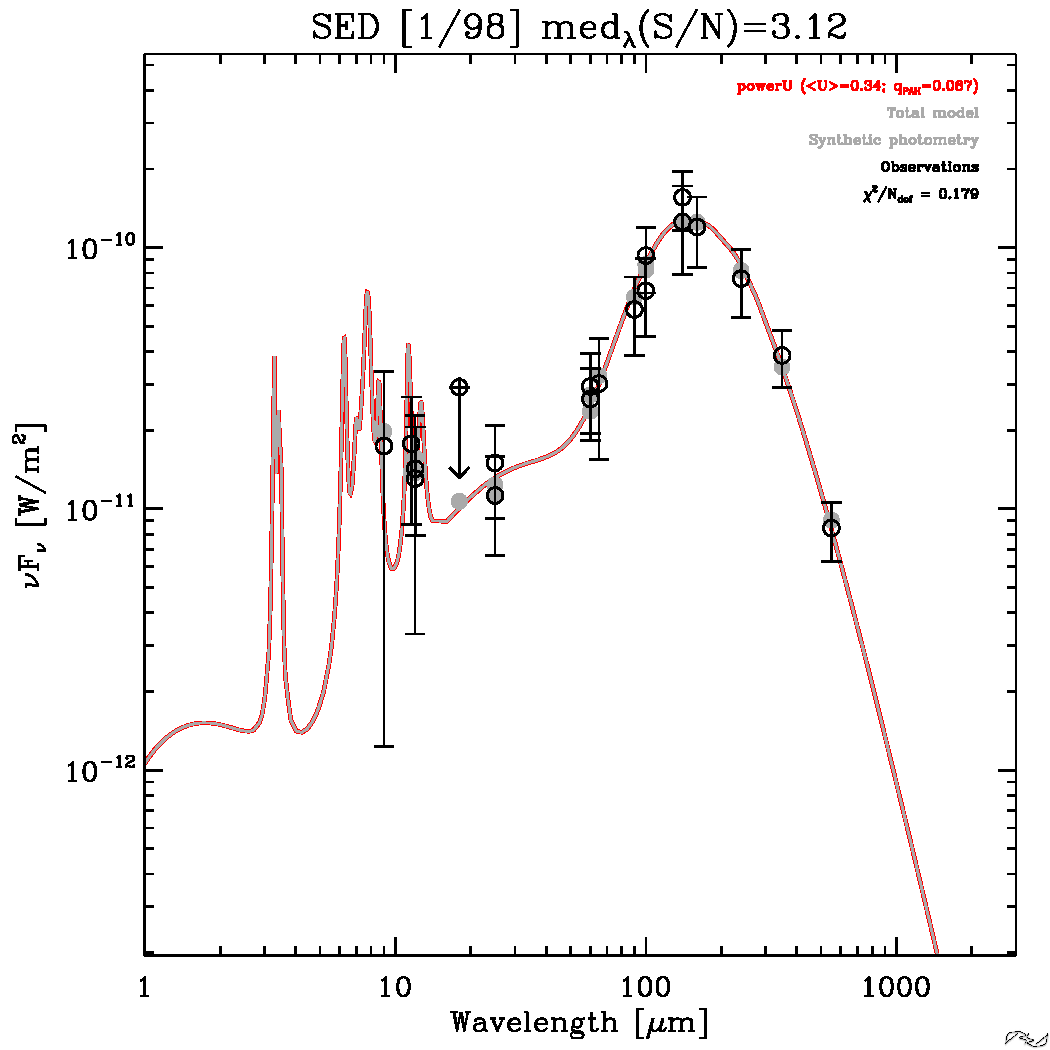
\includegraphics[trim=0 2mm 0 0, clip, width=40mm]{../SEDs/sed_01.pdf}
	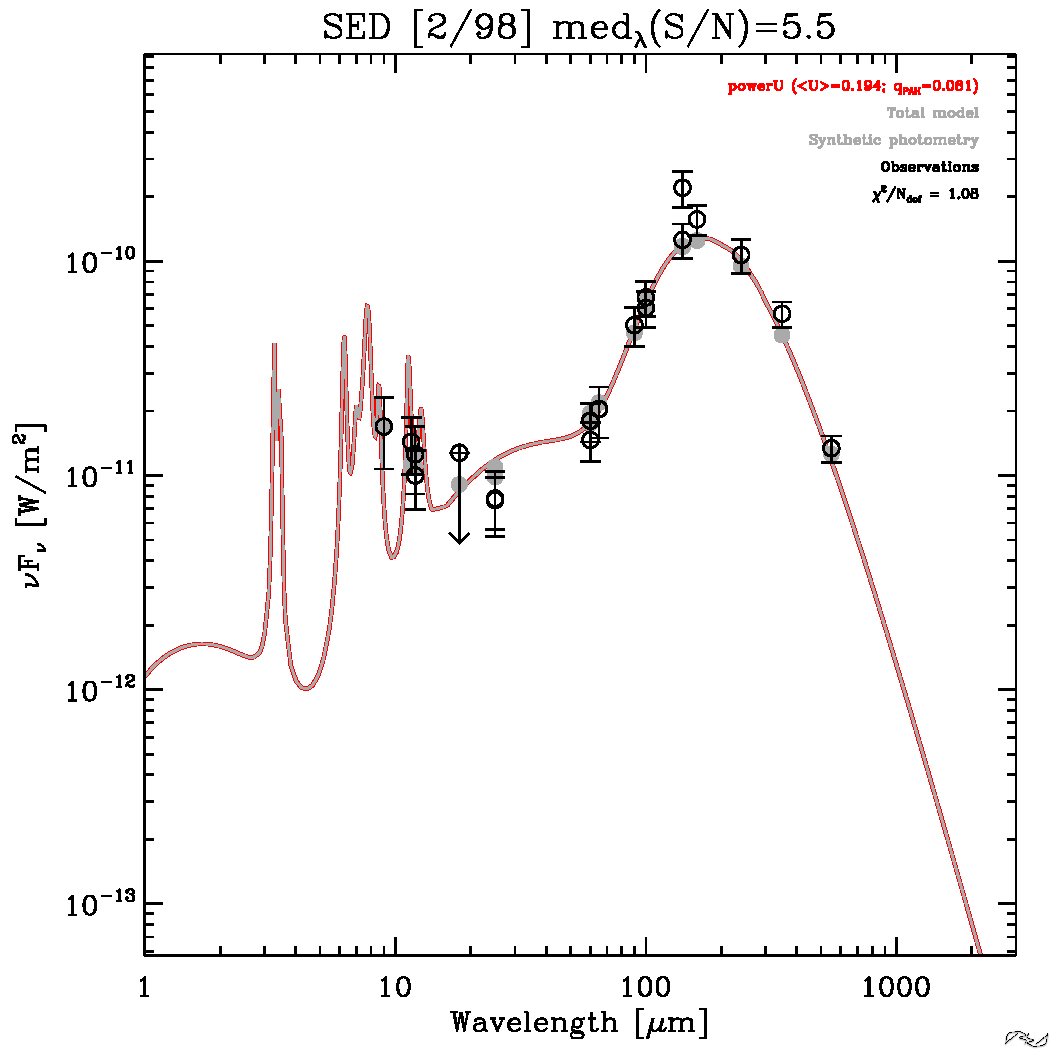
\includegraphics[trim=0 2mm 0 0, clip, width=40mm]{../SEDs/sed_02.pdf}
	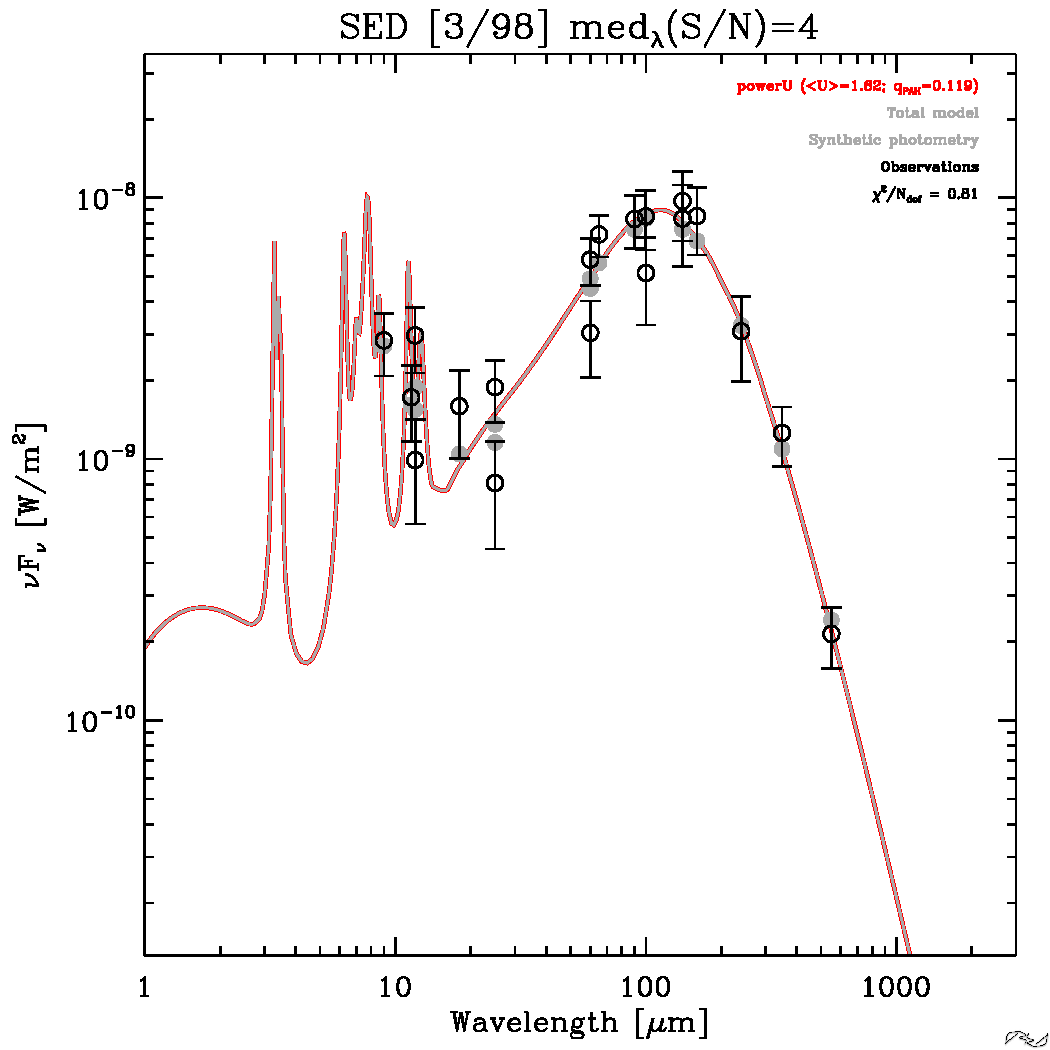
\includegraphics[trim=0 2mm 0 0, clip, width=40mm]{../SEDs/sed_03.pdf}
	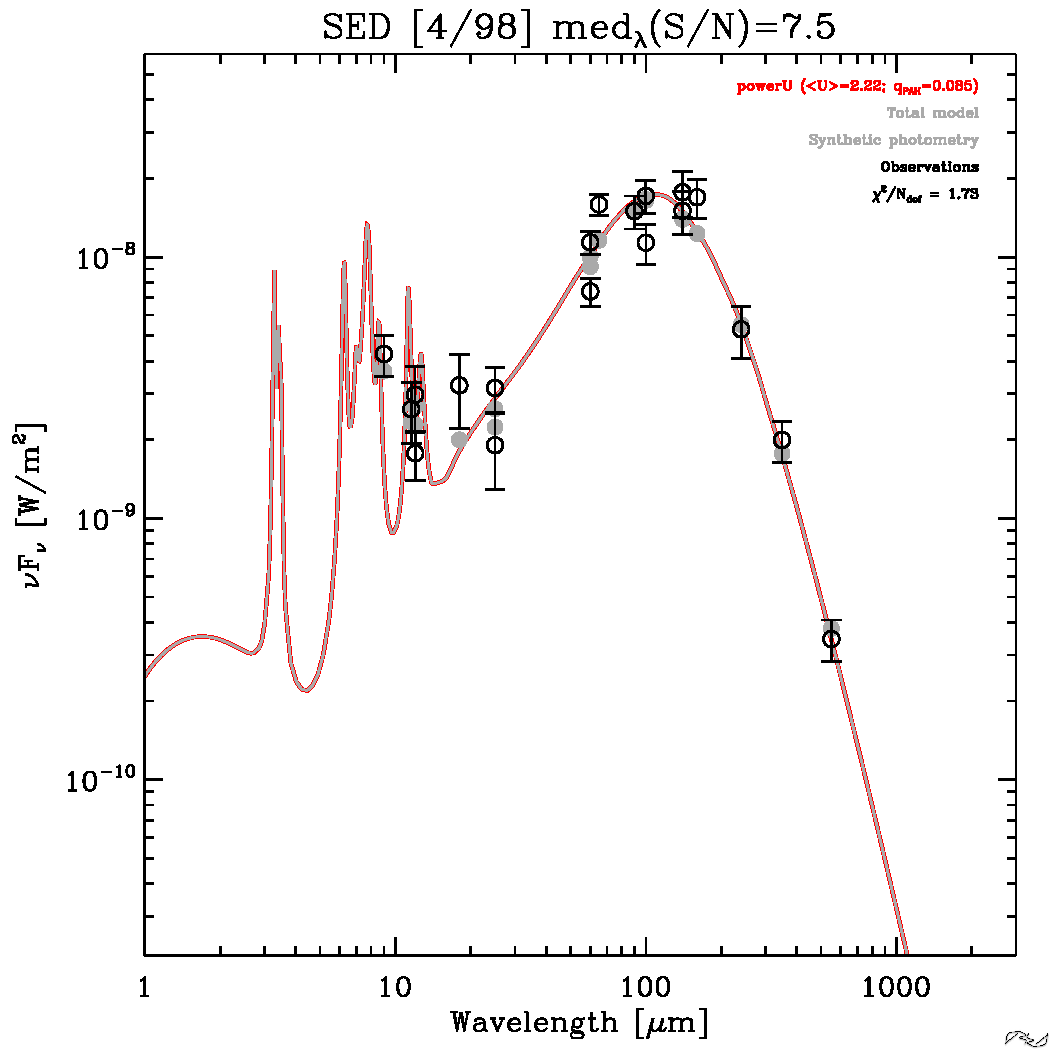
\includegraphics[trim=0 2mm 0 0, clip, width=40mm]{../SEDs/sed_04.pdf}
	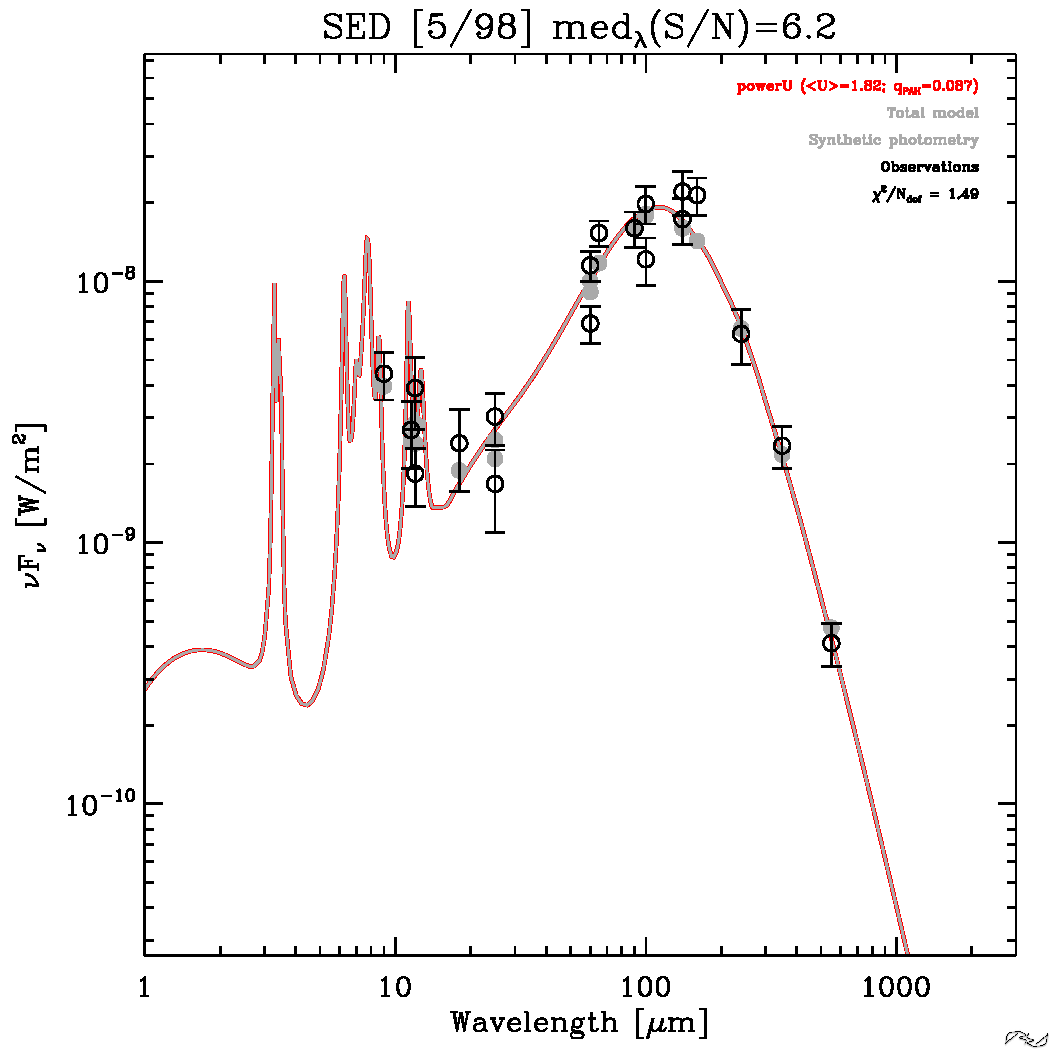
\includegraphics[trim=0 2mm 0 0, clip, width=40mm]{../SEDs/sed_05.pdf}
	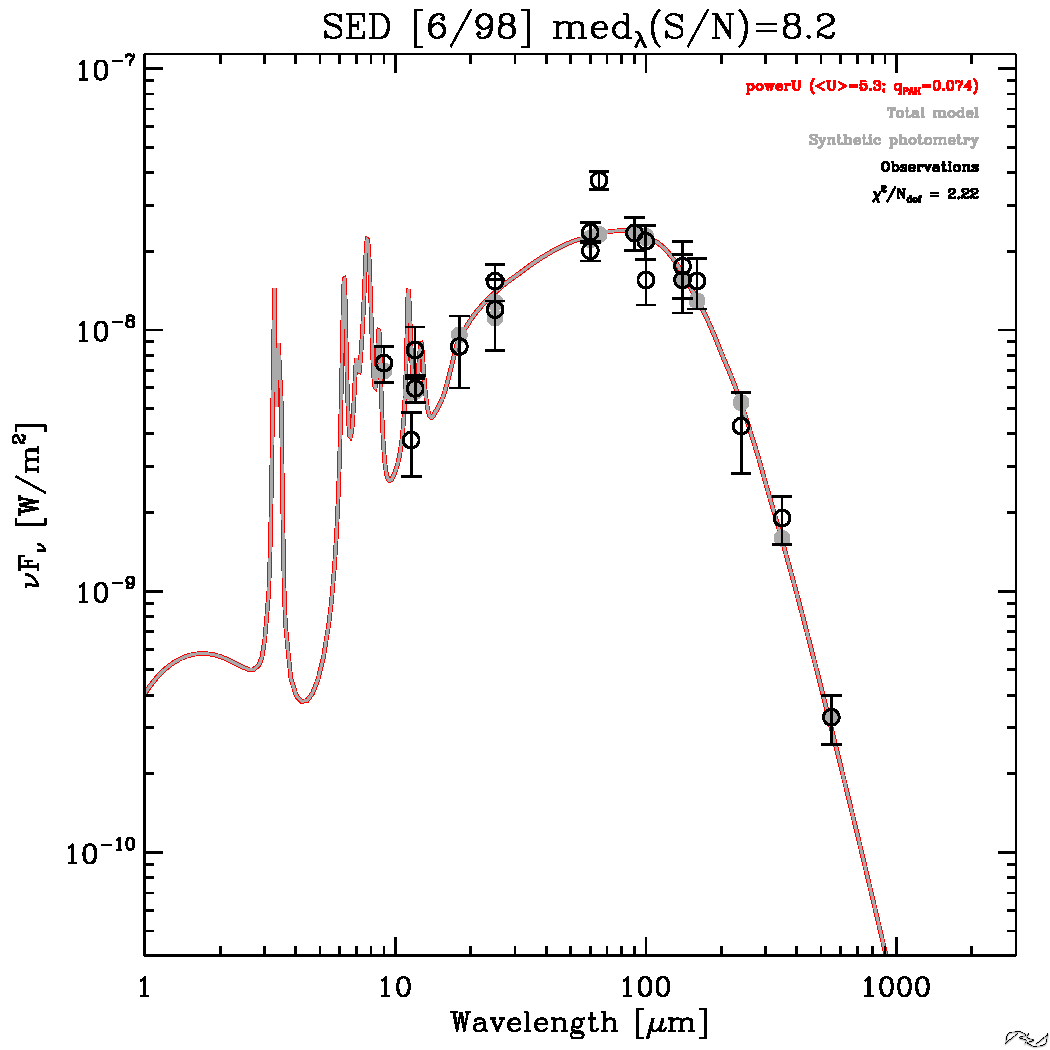
\includegraphics[trim=0 2mm 0 0, clip, width=40mm]{../SEDs/sed_06.pdf}
    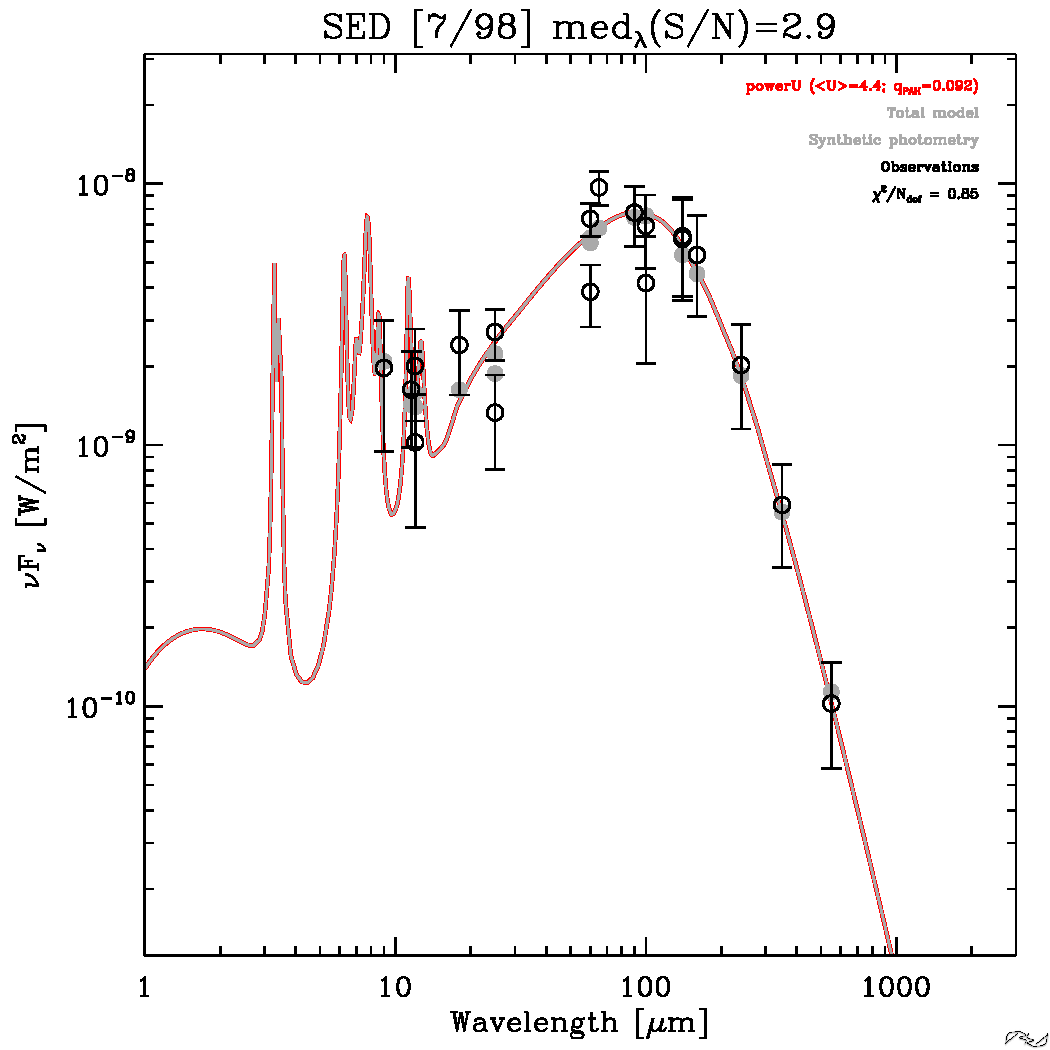
\includegraphics[trim=0 2mm 0 0, clip, width=40mm]{../SEDs/sed_07.pdf}
	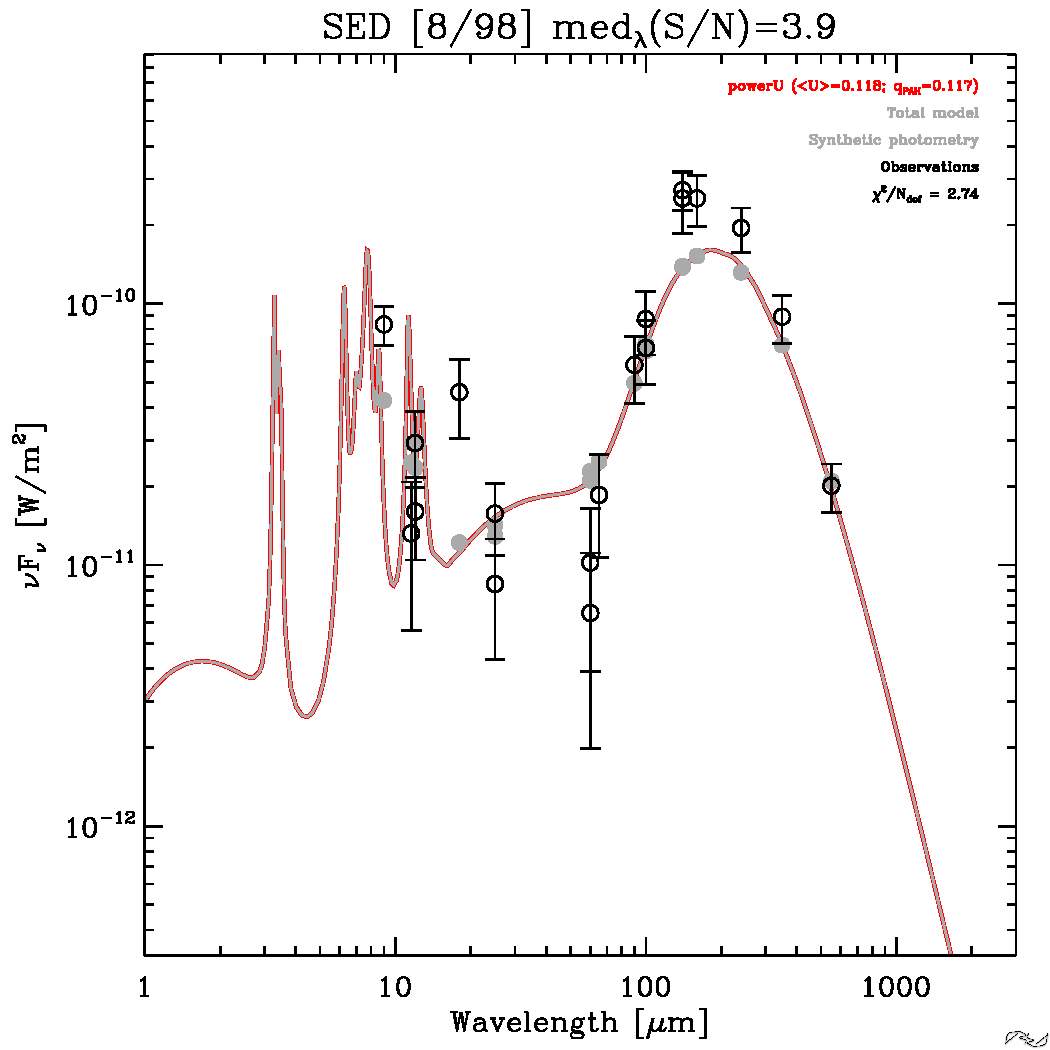
\includegraphics[trim=0 2mm 0 0, clip, width=40mm]{../SEDs/sed_08.pdf}
	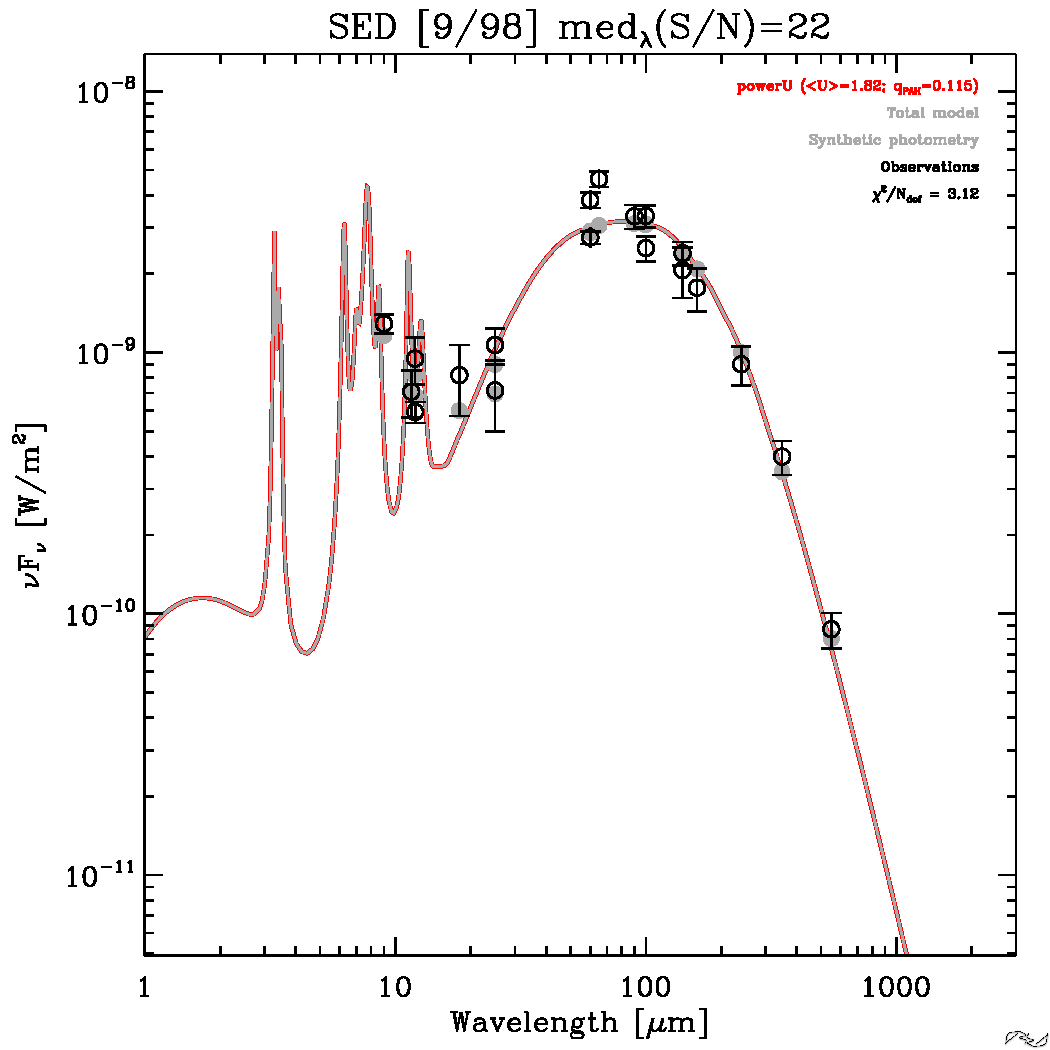
\includegraphics[trim=0 2mm 0 0, clip, width=40mm]{../SEDs/sed_09.pdf}
	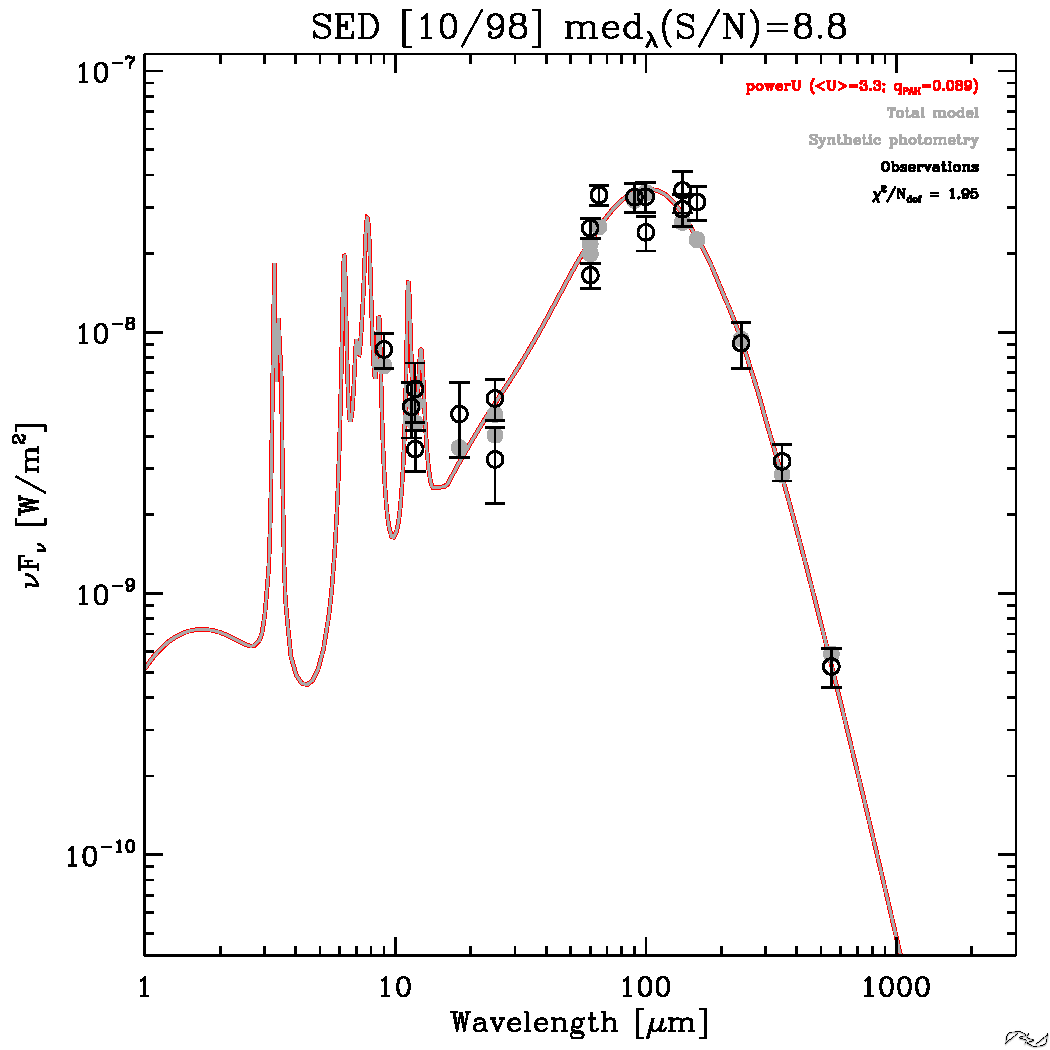
\includegraphics[trim=0 2mm 0 0, clip, width=40mm]{../SEDs/sed_10.pdf}
	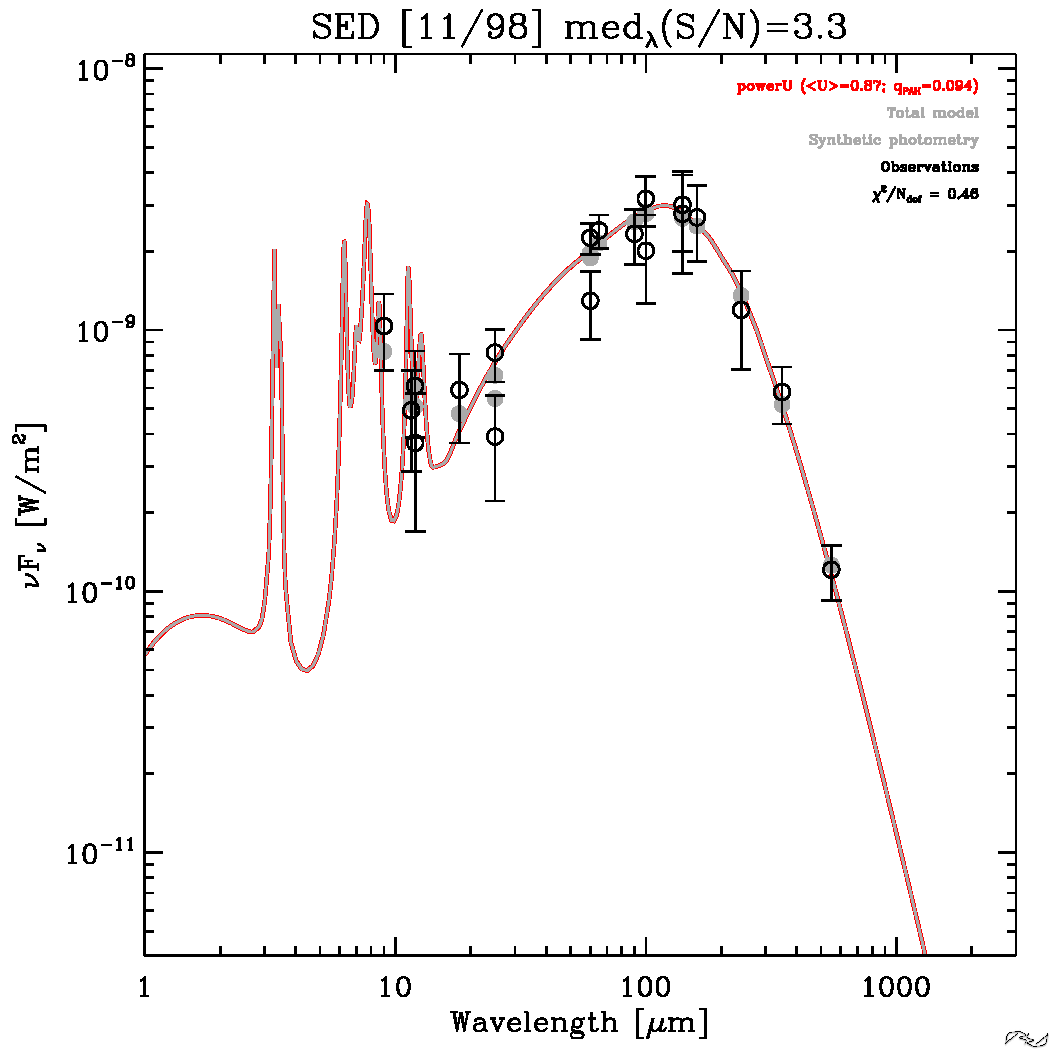
\includegraphics[trim=0 2mm 0 0, clip, width=40mm]{../SEDs/sed_11.pdf}
	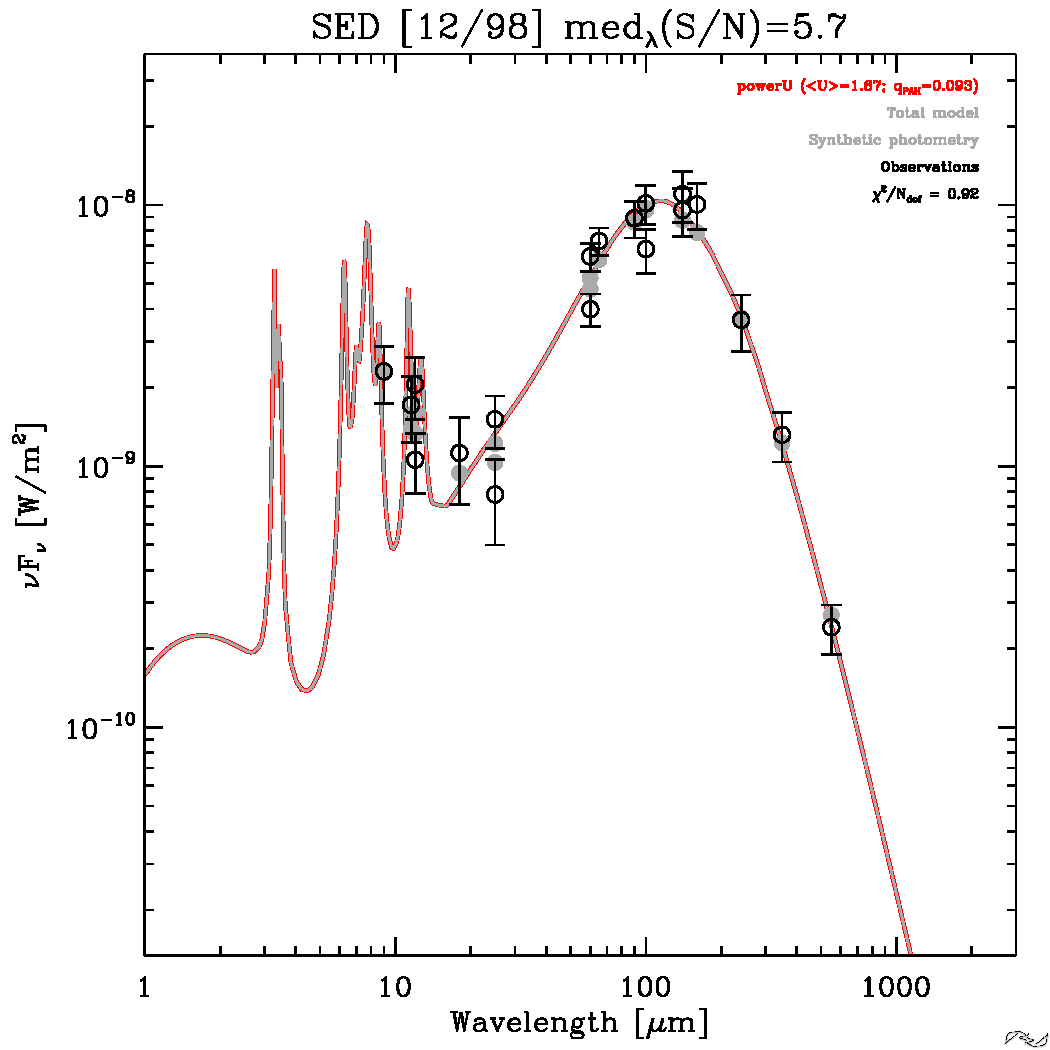
\includegraphics[trim=0 2mm 0 0, clip, width=40mm]{../SEDs/sed_12.pdf}
    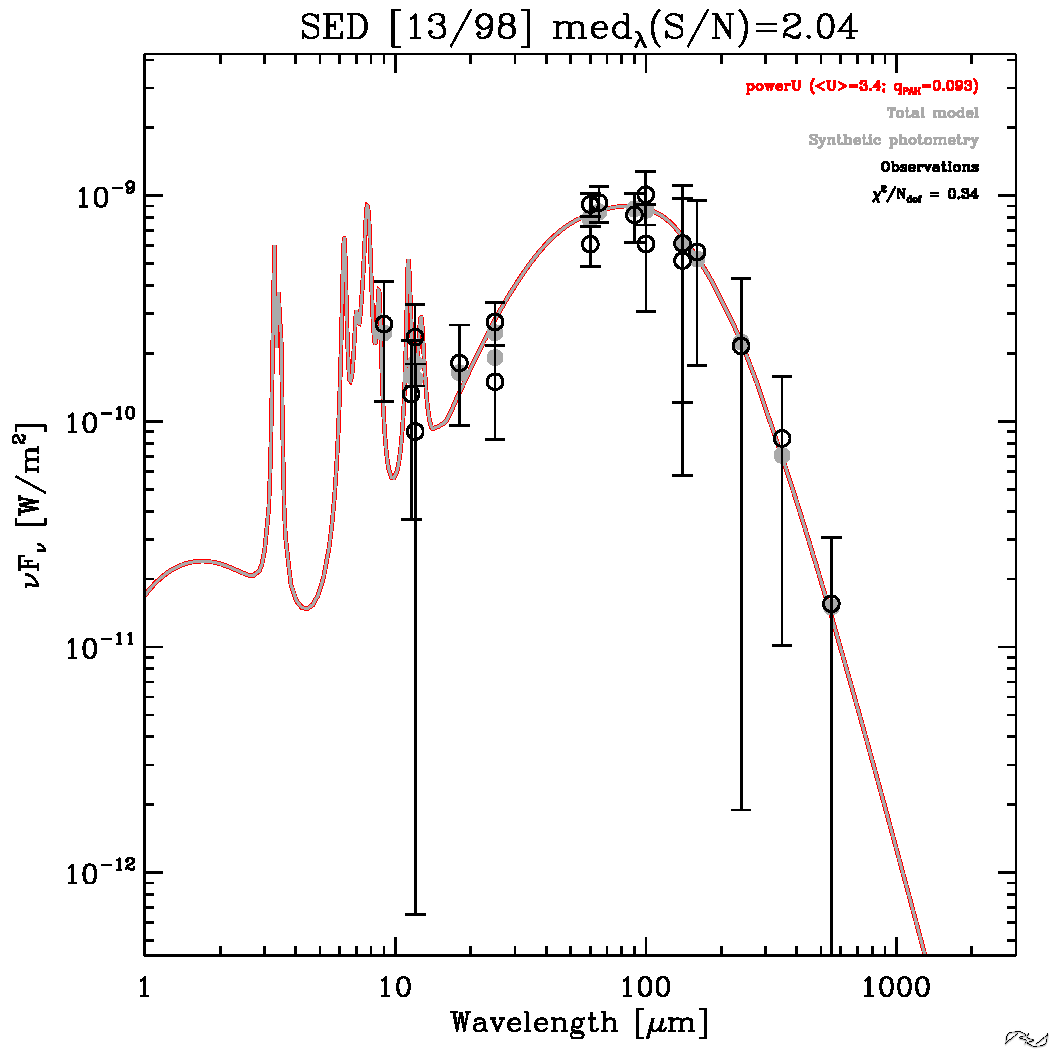
\includegraphics[trim=0 2mm 0 0, clip, width=40mm]{../SEDs/sed_13.pdf}
	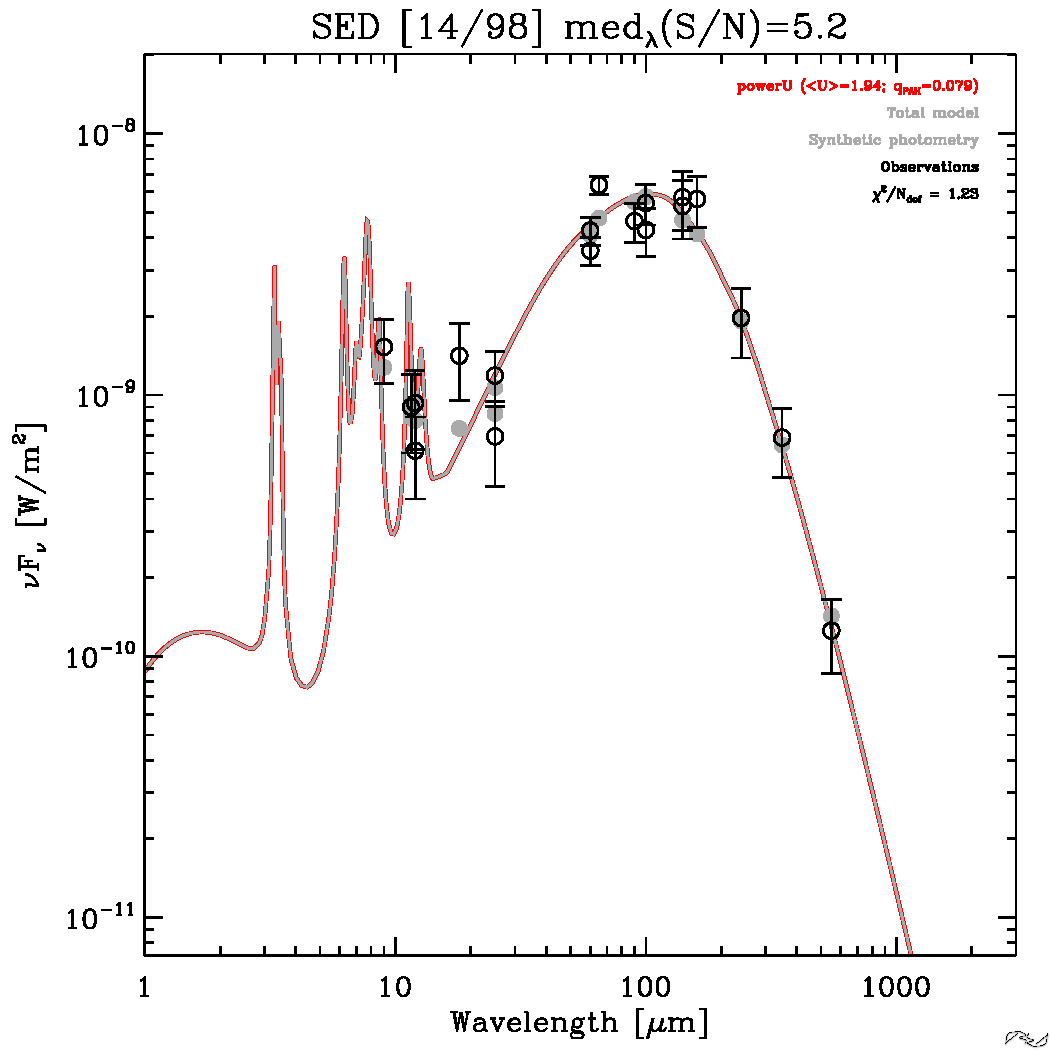
\includegraphics[trim=0 2mm 0 0, clip, width=40mm]{../SEDs/sed_14.pdf}
	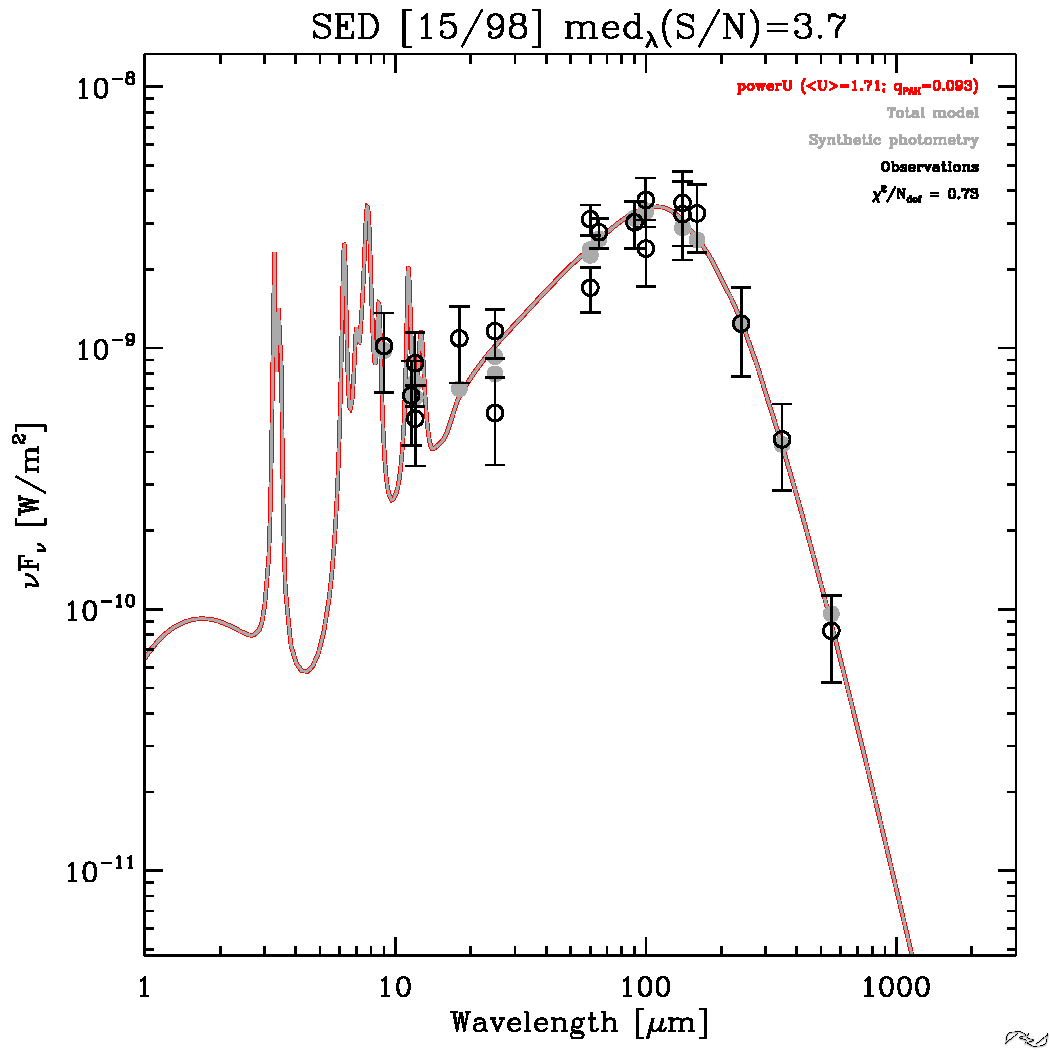
\includegraphics[trim=0 2mm 0 0, clip, width=40mm]{../SEDs/sed_15.pdf}
	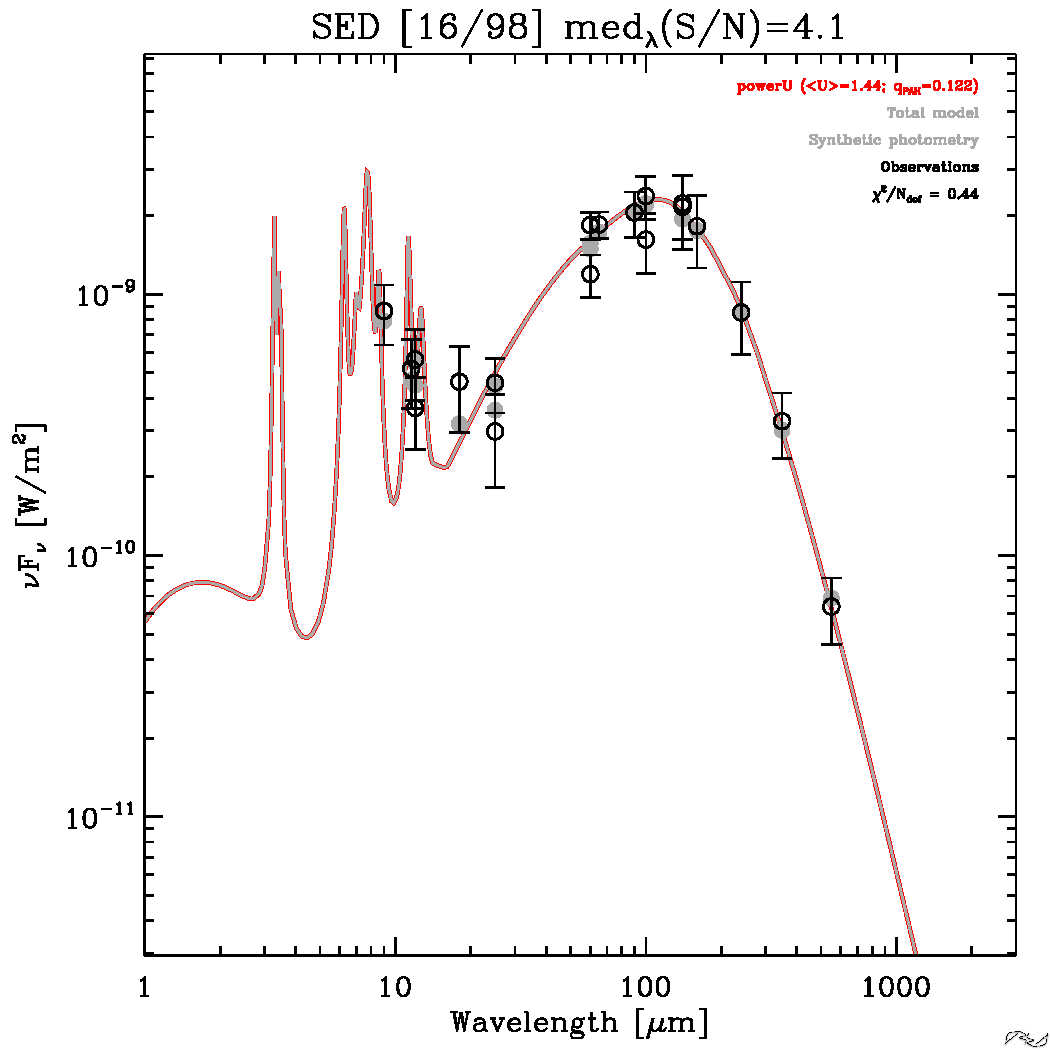
\includegraphics[trim=0 2mm 0 0, clip, width=40mm]{../SEDs/sed_16.pdf}
	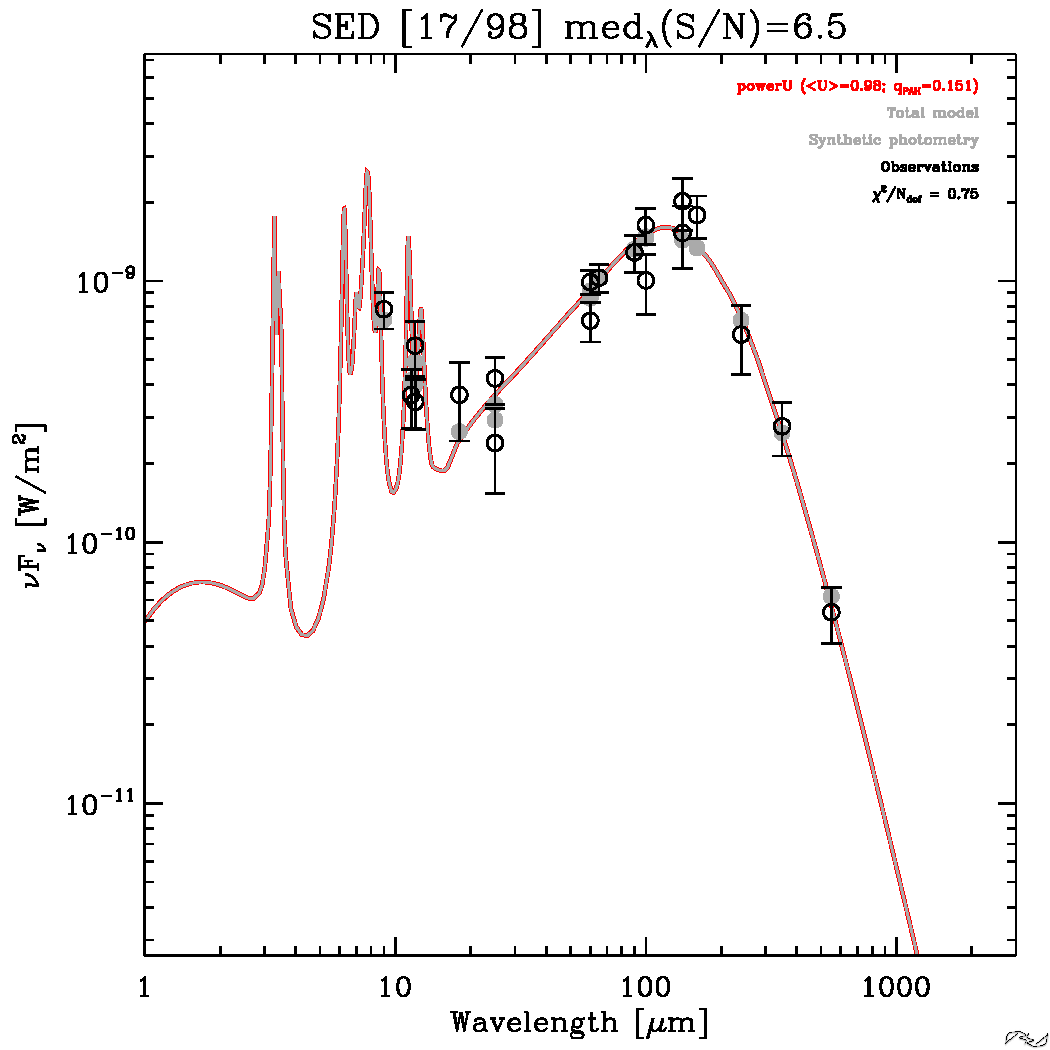
\includegraphics[trim=0 2mm 0 0, clip, width=40mm]{../SEDs/sed_17.pdf}
	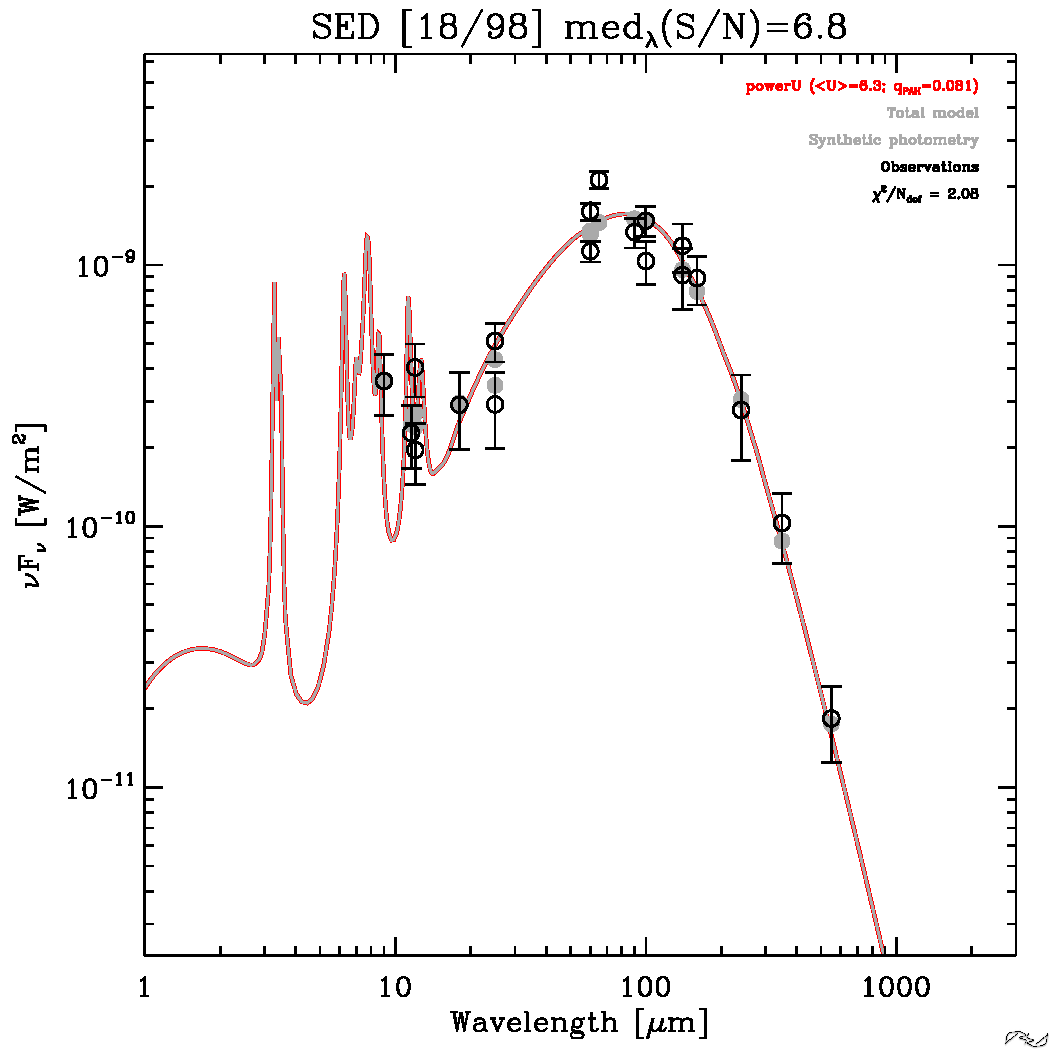
\includegraphics[trim=0 2mm 0 0, clip, width=40mm]{../SEDs/sed_18.pdf}
    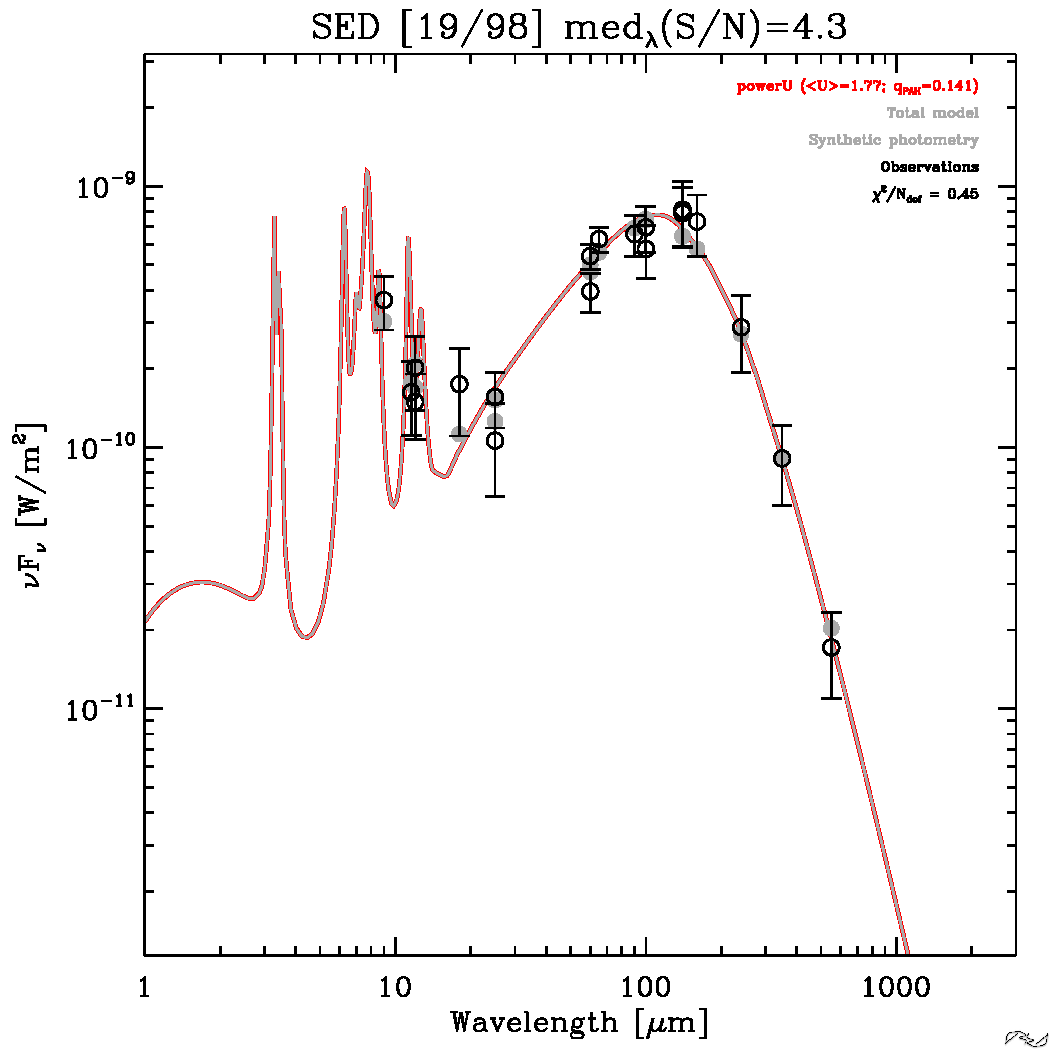
\includegraphics[trim=0 2mm 0 0, clip, width=40mm]{../SEDs/sed_19.pdf}
	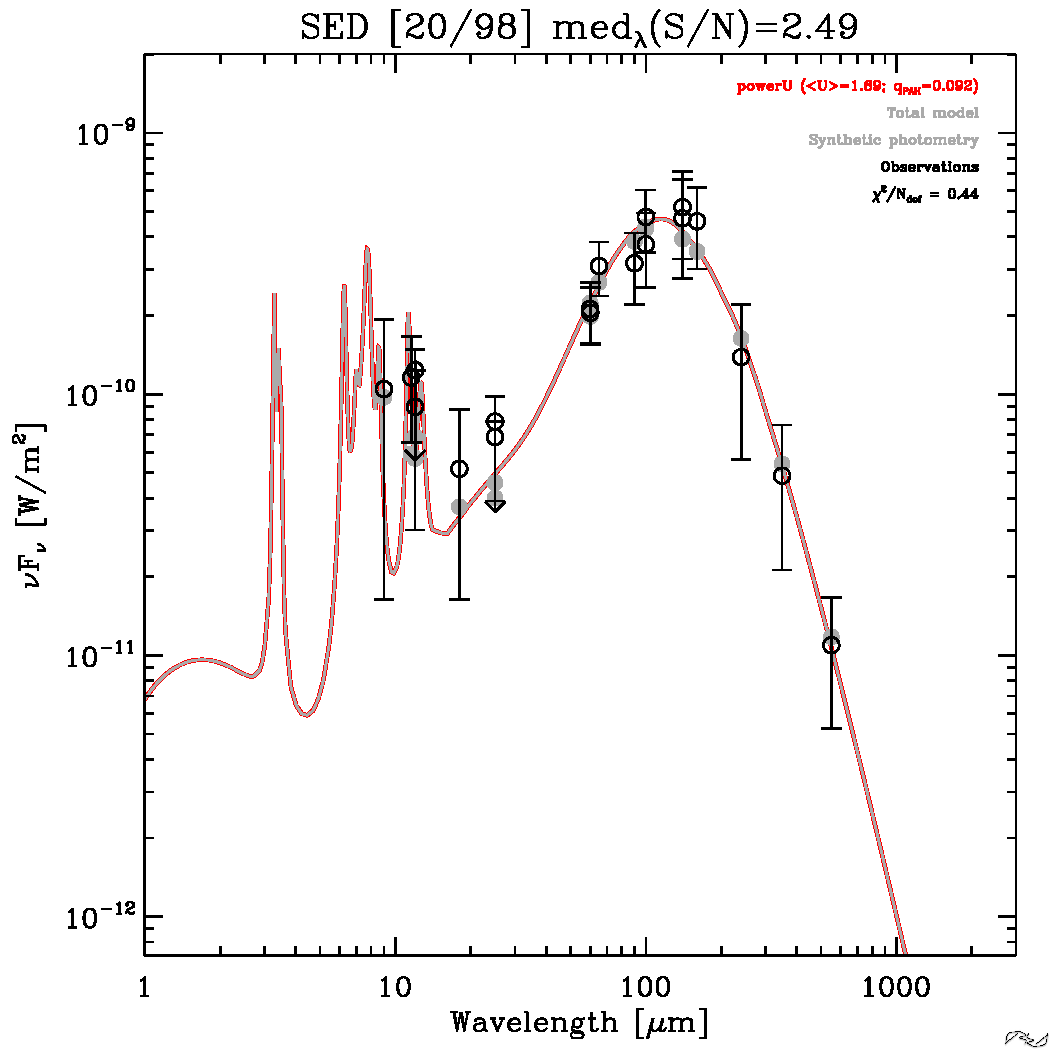
\includegraphics[trim=0 2mm 0 0, clip, width=40mm]{../SEDs/sed_20.pdf}

\end{figure}

\begin{figure}
\centering
    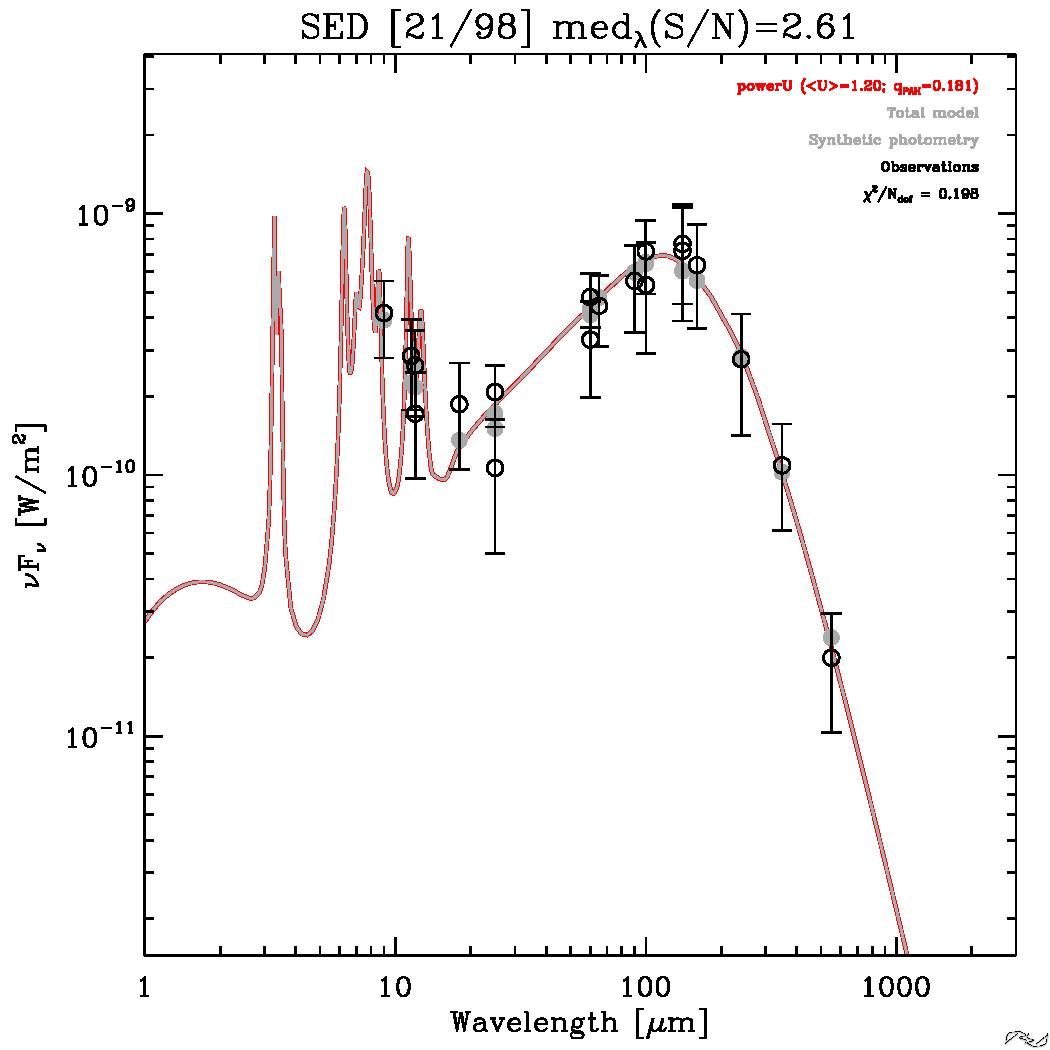
\includegraphics[trim=0 2mm 0 0, clip, width=40mm]{../SEDs/sed_21.pdf}
	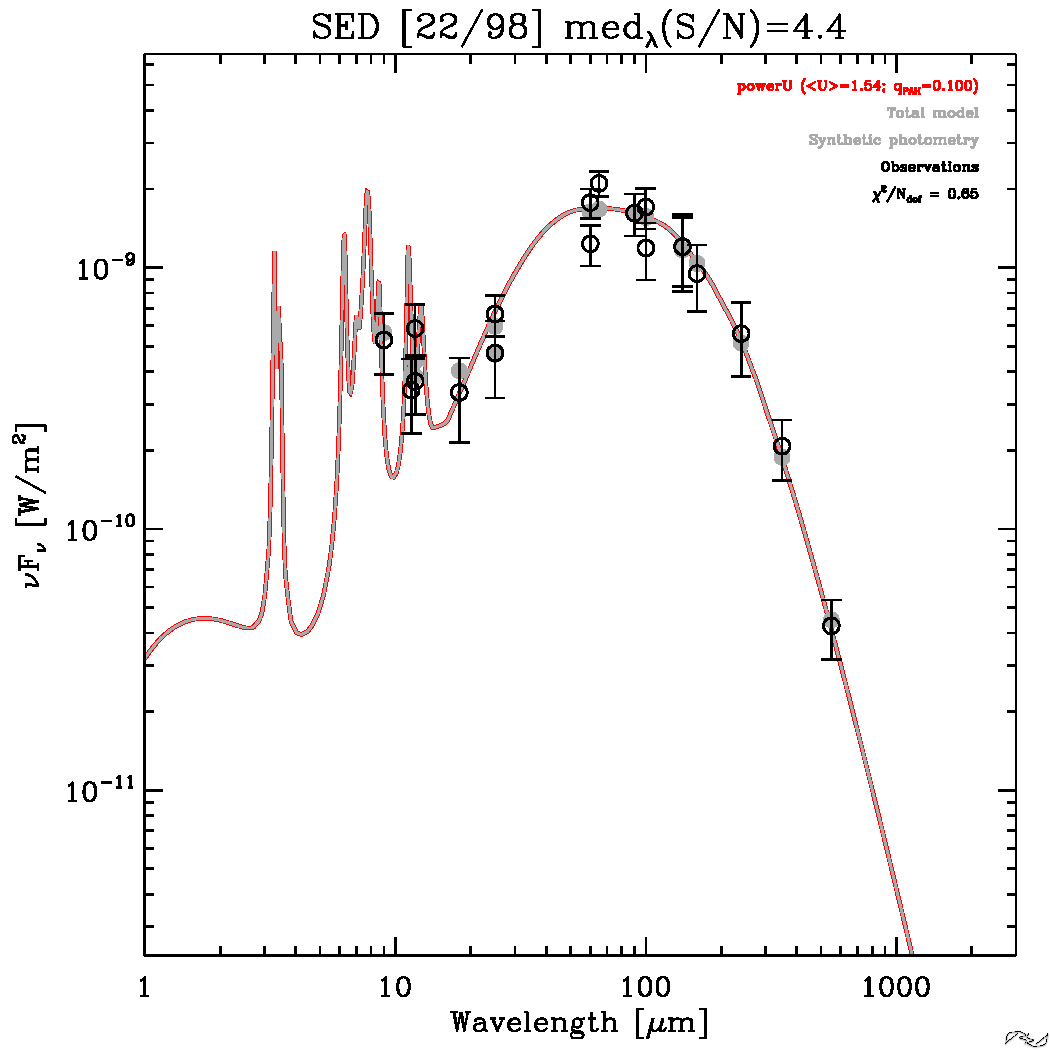
\includegraphics[trim=0 2mm 0 0, clip, width=40mm]{../SEDs/sed_22.pdf}
	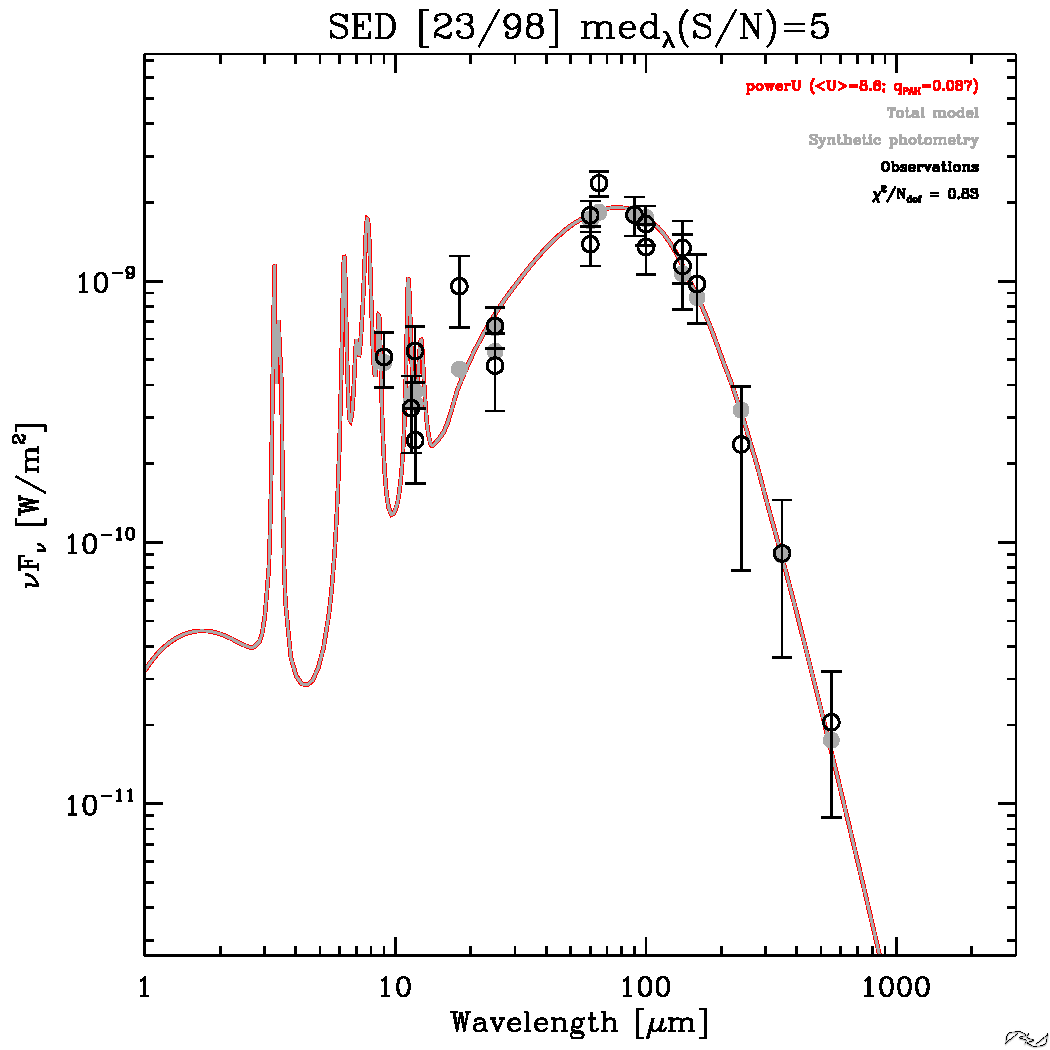
\includegraphics[trim=0 2mm 0 0, clip, width=40mm]{../SEDs/sed_23.pdf}
	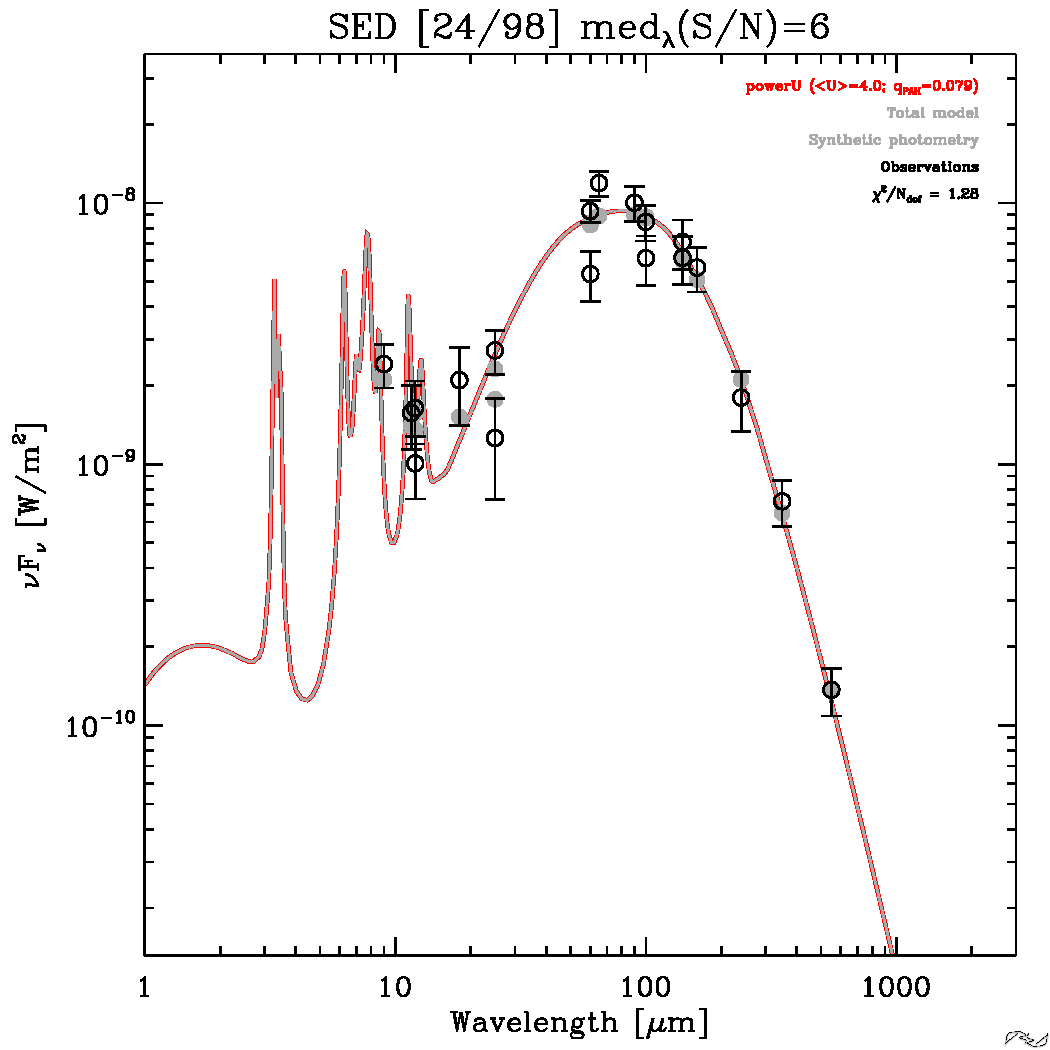
\includegraphics[trim=0 2mm 0 0, clip, width=40mm]{../SEDs/sed_24.pdf}
	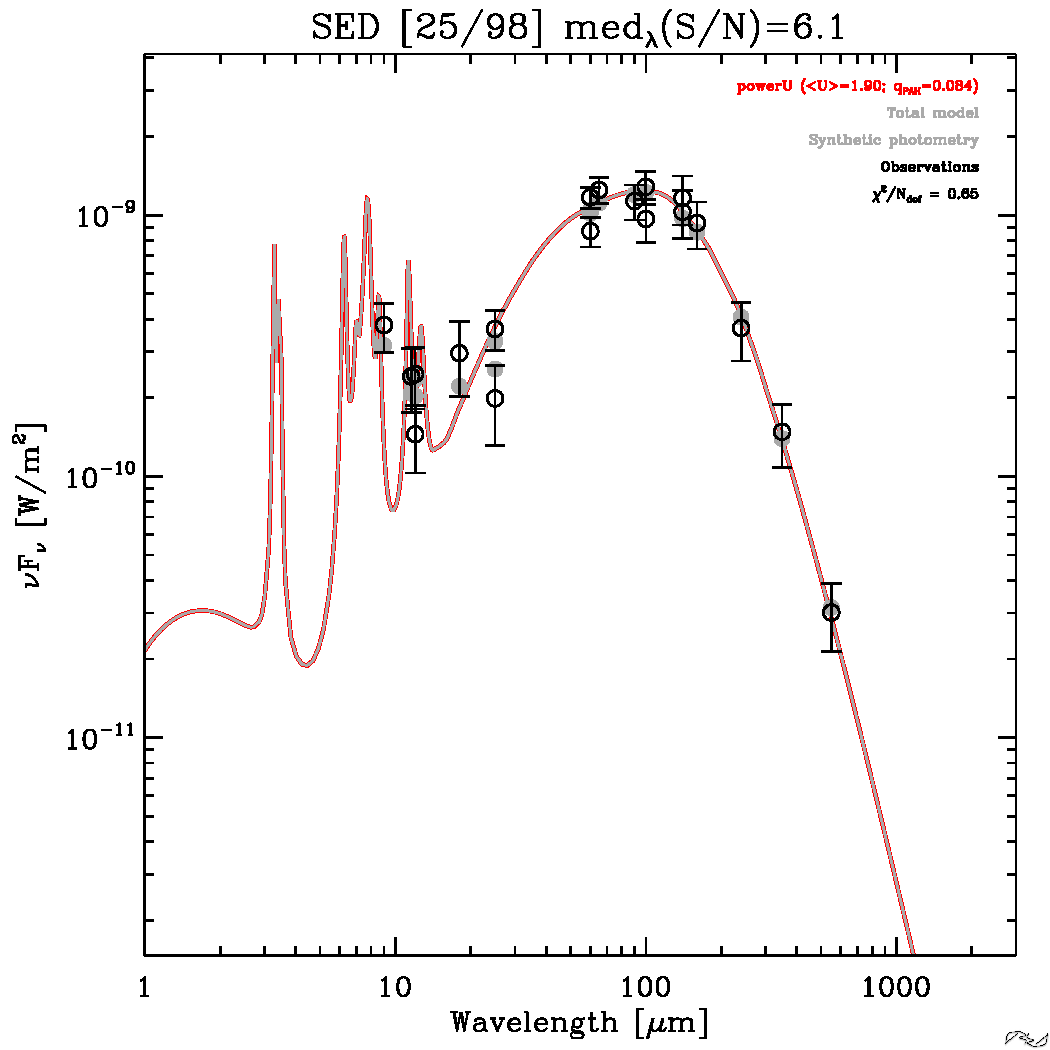
\includegraphics[trim=0 2mm 0 0, clip, width=40mm]{../SEDs/sed_25.pdf}
	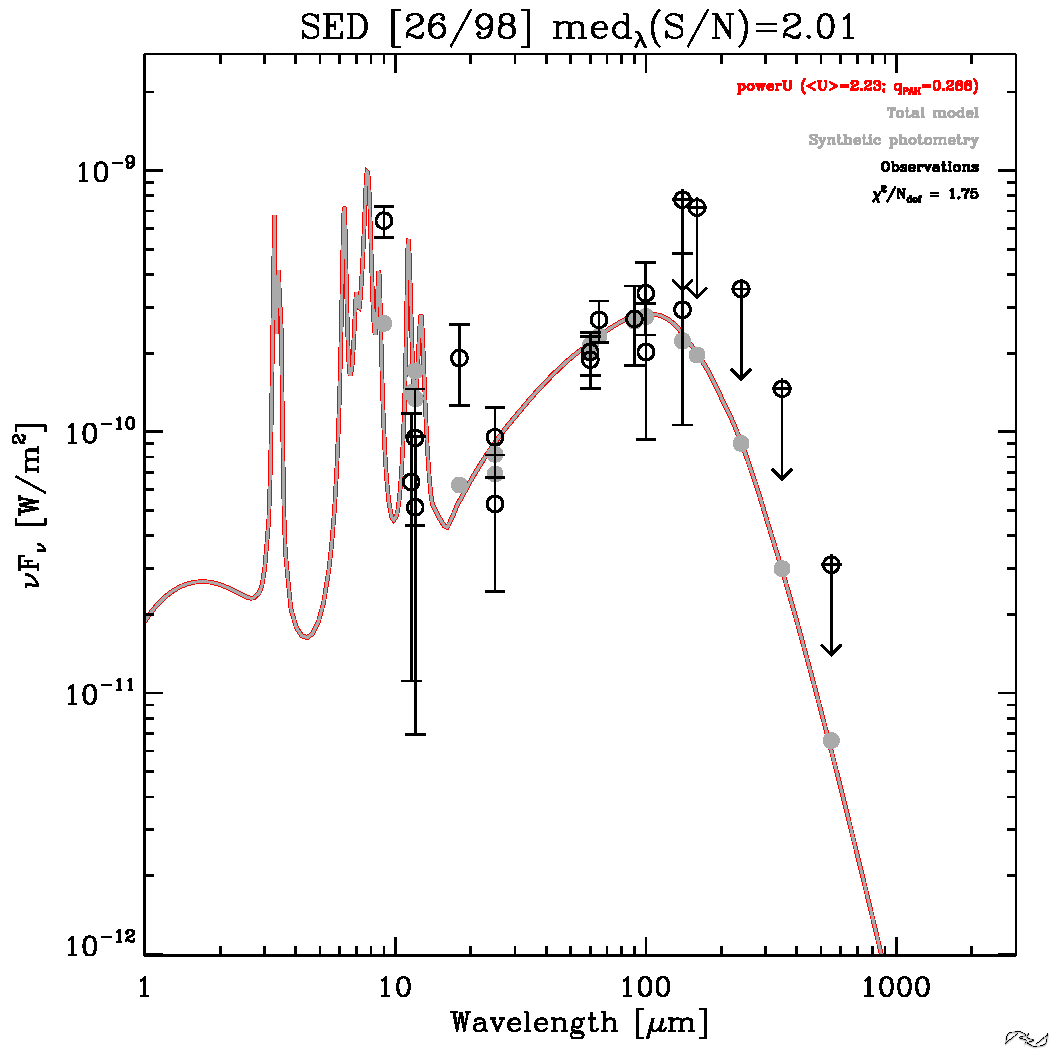
\includegraphics[trim=0 2mm 0 0, clip, width=40mm]{../SEDs/sed_26.pdf}
    \includegraphics[trim=0 2mm 0 0, clip, width=40mm]{../SEDs/sed_27.pdf}
	\includegraphics[trim=0 2mm 0 0, clip, width=40mm]{../SEDs/sed_28.pdf}
	\includegraphics[trim=0 2mm 0 0, clip, width=40mm]{../SEDs/sed_29.pdf}
	\includegraphics[trim=0 2mm 0 0, clip, width=40mm]{../SEDs/sed_30.pdf}
	\includegraphics[trim=0 2mm 0 0, clip, width=40mm]{../SEDs/sed_31.pdf}
	\includegraphics[trim=0 2mm 0 0, clip, width=40mm]{../SEDs/sed_32.pdf}
    \includegraphics[trim=0 2mm 0 0, clip, width=40mm]{../SEDs/sed_33.pdf}
	\includegraphics[trim=0 2mm 0 0, clip, width=40mm]{../SEDs/sed_34.pdf}
	\includegraphics[trim=0 2mm 0 0, clip, width=40mm]{../SEDs/sed_35.pdf}
	\includegraphics[trim=0 2mm 0 0, clip, width=40mm]{../SEDs/sed_36.pdf}
	\includegraphics[trim=0 2mm 0 0, clip, width=40mm]{../SEDs/sed_37.pdf}
	\includegraphics[trim=0 2mm 0 0, clip, width=40mm]{../SEDs/sed_38.pdf}
    \includegraphics[trim=0 2mm 0 0, clip, width=40mm]{../SEDs/sed_39.pdf}
	\includegraphics[trim=0 2mm 0 0, clip, width=40mm]{../SEDs/sed_40.pdf}
\end{figure}

\begin{figure}
\centering
    \includegraphics[trim=0 2mm 0 0, clip, width=40mm]{../SEDs/sed_41.pdf}
	\includegraphics[trim=0 2mm 0 0, clip, width=40mm]{../SEDs/sed_42.pdf}
	\includegraphics[trim=0 2mm 0 0, clip, width=40mm]{../SEDs/sed_43.pdf}
	\includegraphics[trim=0 2mm 0 0, clip, width=40mm]{../SEDs/sed_44.pdf}
	\includegraphics[trim=0 2mm 0 0, clip, width=40mm]{../SEDs/sed_45.pdf}
	\includegraphics[trim=0 2mm 0 0, clip, width=40mm]{../SEDs/sed_46.pdf}
    \includegraphics[trim=0 2mm 0 0, clip, width=40mm]{../SEDs/sed_47.pdf}
	\includegraphics[trim=0 2mm 0 0, clip, width=40mm]{../SEDs/sed_48.pdf}
	\includegraphics[trim=0 2mm 0 0, clip, width=40mm]{../SEDs/sed_49.pdf}
	\includegraphics[trim=0 2mm 0 0, clip, width=40mm]{../SEDs/sed_50.pdf}
	\includegraphics[trim=0 2mm 0 0, clip, width=40mm]{../SEDs/sed_51.pdf}
	\includegraphics[trim=0 2mm 0 0, clip, width=40mm]{../SEDs/sed_52.pdf}
    \includegraphics[trim=0 2mm 0 0, clip, width=40mm]{../SEDs/sed_53.pdf}
	\includegraphics[trim=0 2mm 0 0, clip, width=40mm]{../SEDs/sed_54.pdf}
	\includegraphics[trim=0 2mm 0 0, clip, width=40mm]{../SEDs/sed_55.pdf}
	\includegraphics[trim=0 2mm 0 0, clip, width=40mm]{../SEDs/sed_56.pdf}
	\includegraphics[trim=0 2mm 0 0, clip, width=40mm]{../SEDs/sed_57.pdf}
	\includegraphics[trim=0 2mm 0 0, clip, width=40mm]{../SEDs/sed_58.pdf}
    \includegraphics[trim=0 2mm 0 0, clip, width=40mm]{../SEDs/sed_59.pdf}
	\includegraphics[trim=0 2mm 0 0, clip, width=40mm]{../SEDs/sed_60.pdf}
\end{figure}
\begin{figure}
\centering
    \includegraphics[trim=0 2mm 0 0, clip, width=40mm]{../SEDs/sed_61.pdf}
	\includegraphics[trim=0 2mm 0 0, clip, width=40mm]{../SEDs/sed_62.pdf}
	\includegraphics[trim=0 2mm 0 0, clip, width=40mm]{../SEDs/sed_63.pdf}
	\includegraphics[trim=0 2mm 0 0, clip, width=40mm]{../SEDs/sed_64.pdf}
	\includegraphics[trim=0 2mm 0 0, clip, width=40mm]{../SEDs/sed_65.pdf}
	\includegraphics[trim=0 2mm 0 0, clip, width=40mm]{../SEDs/sed_66.pdf}
    \includegraphics[trim=0 2mm 0 0, clip, width=40mm]{../SEDs/sed_67.pdf}
	\includegraphics[trim=0 2mm 0 0, clip, width=40mm]{../SEDs/sed_68.pdf}
	\includegraphics[trim=0 2mm 0 0, clip, width=40mm]{../SEDs/sed_69.pdf}
	\includegraphics[trim=0 2mm 0 0, clip, width=40mm]{../SEDs/sed_70.pdf}
	\includegraphics[trim=0 2mm 0 0, clip, width=40mm]{../SEDs/sed_71.pdf}
	\includegraphics[trim=0 2mm 0 0, clip, width=40mm]{../SEDs/sed_72.pdf}
    \includegraphics[trim=0 2mm 0 0, clip, width=40mm]{../SEDs/sed_73.pdf}
	\includegraphics[trim=0 2mm 0 0, clip, width=40mm]{../SEDs/sed_74.pdf}
	\includegraphics[trim=0 2mm 0 0, clip, width=40mm]{../SEDs/sed_75.pdf}
	\includegraphics[trim=0 2mm 0 0, clip, width=40mm]{../SEDs/sed_76.pdf}
	\includegraphics[trim=0 2mm 0 0, clip, width=40mm]{../SEDs/sed_77.pdf}
	\includegraphics[trim=0 2mm 0 0, clip, width=40mm]{../SEDs/sed_78.pdf}
    \includegraphics[trim=0 2mm 0 0, clip, width=40mm]{../SEDs/sed_79.pdf}
	\includegraphics[trim=0 2mm 0 0, clip, width=40mm]{../SEDs/sed_80.pdf}
\end{figure}
\begin{figure}
\centering
    \includegraphics[trim=0 2mm 0 0, clip, width=40mm]{../SEDs/sed_81.pdf}
	\includegraphics[trim=0 2mm 0 0, clip, width=40mm]{../SEDs/sed_82.pdf}
	\includegraphics[trim=0 2mm 0 0, clip, width=40mm]{../SEDs/sed_83.pdf}
	\includegraphics[trim=0 2mm 0 0, clip, width=40mm]{../SEDs/sed_84.pdf}
	\includegraphics[trim=0 2mm 0 0, clip, width=40mm]{../SEDs/sed_85.pdf}
	\includegraphics[trim=0 2mm 0 0, clip, width=40mm]{../SEDs/sed_86.pdf}
    \includegraphics[trim=0 2mm 0 0, clip, width=40mm]{../SEDs/sed_87.pdf}
	\includegraphics[trim=0 2mm 0 0, clip, width=40mm]{../SEDs/sed_88.pdf}
	\includegraphics[trim=0 2mm 0 0, clip, width=40mm]{../SEDs/sed_89.pdf}
	\includegraphics[trim=0 2mm 0 0, clip, width=40mm]{../SEDs/sed_90.pdf}
	\includegraphics[trim=0 2mm 0 0, clip, width=40mm]{../SEDs/sed_91.pdf}
	\includegraphics[trim=0 2mm 0 0, clip, width=40mm]{../SEDs/sed_92.pdf}
    \includegraphics[trim=0 2mm 0 0, clip, width=40mm]{../SEDs/sed_93.pdf}
	\includegraphics[trim=0 2mm 0 0, clip, width=40mm]{../SEDs/sed_94.pdf}
	\includegraphics[trim=0 2mm 0 0, clip, width=40mm]{../SEDs/sed_95.pdf}
	\includegraphics[trim=0 2mm 0 0, clip, width=40mm]{../SEDs/sed_96.pdf}
	\includegraphics[trim=0 2mm 0 0, clip, width=40mm]{../SEDs/sed_97.pdf}
	\includegraphics[trim=0 2mm 0 0, clip, width=40mm]{../SEDs/sed_98.pdf}
\end{figure}

%\fi

\small
\bibliographystyle{apj}
\bibliography{reference}

\end{document}
